\documentclass[12pt,twoside]{report}
\usepackage[a4paper,top=3cm,bottom=2cm, left=3cm, right=2cm]{geometry}
\usepackage[utf8]{inputenc}
\usepackage{listings}
\usepackage{graphicx}
\usepackage{mathdots}
\usepackage{tikz}
\usepackage{booktabs}
\usepackage{pgffor} 
\usepackage{float}
\usepackage{graphics} 
\usepackage{fancyhdr}
\usepackage[square, sort, numbers]{natbib}
\usepackage{color}
\usepackage{indentfirst}
\usepackage{epigraph}
\usepackage{ragged2e}
\usepackage{blindtext}
\usepackage{amsmath,amsthm,amssymb}
\usepackage{tabto}
\usepackage{pgfplots}
\usepackage{changepage}
\usepackage{subcaption}
\usepackage{fancyvrb}
\usepackage{caption}
\usepackage{minted}
\usepackage{placeins} % put this in your pre-amble
\usepackage{flafter}  % put this in your pre-amble

\usetikzlibrary{patterns}
\usetikzlibrary{arrows.meta}

\graphicspath{{images/}}

\definecolor{mycolor}{RGB}{30,75,180}
\definecolor{mycolor2}{RGB}{40,75,90}
\definecolor{red}{RGB}{200,0,0}
\usepackage[colorlinks = true,
            linkcolor = mycolor,
            urlcolor  = mycolor,
            citecolor = mycolor,
            anchorcolor = mycolor]{hyperref}

\usepackage[hypcap=true,font={small,it}]{caption}
\usetikzlibrary{calc}

\captionsetup{belowskip=2pt,aboveskip=2pt}

\bibliographystyle{abstract}

\renewcommand{\chaptername}{}

\renewcommand{\figureautorefname}{figure} % lower case default ref
\renewcommand{\tableautorefname}{table} % lower case default ref
\let\oldchapter\chapter% Store \section in \oldsection
\renewcommand{\chapter}{\cleardoublepage\oldchapter}% Prepend new \section with \cleardoublepage

\newcommand{\latex}{\LaTeX\xspace}
\newcommand{\mcite}[1]{\textcolor{mycolor}{\citeauthor{#1} (\citeyear{#1})}}
\newcommand{\hcite}[1]{(\textcolor{mycolor}{\citeauthor{#1}, \citeyear{#1}})}
\newcommand{\defi}[1]{\textbf{#1}}
\newcommand{\naming}[1]{\textbf{#1}}
\newcommand{\todo}[1]{\textbf{\color{red} TODO: #1}}
\newcommand{\gam}[2]{\mbox{$\{#1\:|\:#2\}$}}
\newcommand{\Gm}[1]{\mbox{$G#1$}}
\newcommand{\Hm}{\mbox{$H\,$}}

\definecolor{purple2}{RGB}{218,112,214}

\pgfplotsset{style thermograph/.style={
		axis x line*=none, axis y line*=none,
		axis line style={draw=none},
		y label style={rotate=-90,at={(current axis.north west)}, right=5mm},
		ylabel = \textbf{t},
	}
}
\lstset{
	columns=fullflexible,
	mathescape=true,
	numbers=none,
	stepnumber=1,
	morekeywords={return, if, else,  while, vector, using, include, class,
		true, false, function, or, public, private},
	xleftmargin=4.0ex,
	tabsize=4,
	frame = single
}


%----------------------------------------------------------------------------------------------------%

%--------------------------------------------- DOCUMENT ---------------------------------------------%
\begin{document}
	\newpage
    \begin{titlepage}
\vspace*{-2.5cm}
\begin{figure}[H]
    \hspace*{-1.0cm}
    \vspace*{-0.5cm}
    
\includegraphics[scale=0.4]{images/logo_ime.png}\\
\end{figure}

\noindent Universidade de São Paulo - Instituto de Matemática e Estatística\\
Bachelor's Programme in Computer Science
    \begin{center}
        \vspace*{1cm}
        
        {\LARGE \textbf{HOT GAMES}}
        
        \vspace{0.5cm}
        Temperature, advantage and numbers
        
        \vspace{1.5cm}
        by \\
        \vspace{1.5cm}
       Matheus Tararam de Laurentys
                
        \vspace{1.0cm}
    \end{center}

\noindent{
\textcolor{red}{{\bf Abstract} (The Abstract is a short summary of what your thesis is about. It accurately reflects the content of the thesis providing information about the research problem, research aims, methods and procedures, results and implications. It is a short section. Abstracts give readers the opportunity to quickly see the main contents of the paper and enable them to decide whether the paper is of particular interest to their needs. This section will be one of the last sections that you write. No subheadings are used in an abstract.)
}
}
\vfill
\textcolor[rgb]{0.5,0.5,0.5}{
    \begin{flushleft}
    { \small
    MAC0499 \\
    Undergraduate Thesis \\
    (Month) (Year) \\
    Supervisor: José Coelho Pina \\
    }
    \end{flushleft}
}
      
\end{titlepage}

    \newpage

{
\noindent\Large\textbf{Abstract}
}\\


\noindent
Combinatorial games are called hot when their position is active, meaning that both players want to make the next move. Hot games are the ones that typically lead to interesting play. Before focusing in this class of games, the text will present fundamental ideas for their study. The first three chapters present and explain the concepts involved with the analysis of combinatorial games. In this first half, there is great concern with the correspondence between games and numbers and how games might or might not be numbers.

The fourth chapter formalizes the idea of temperature and provides methods to handle hot games. The following chapter make use of all content to provide insight into more advanced ideas and discuss basic applications of the definitions. The sixth chapter, then, works the way up to the proof of a most important theorem and provides its result for a game that permeates the text, Domineering. The text finishes by providing some of the possible next steps, areas that were not discussed and pointing to a few references.

\newpage

{
\noindent\Large\textbf{Resumo}
}\\


\noindent
Jogos combinatórios são chamados quentes quando suas posições são ativas, o que significa que ambos os jogadores querem fazer o próximo movimento. Jogos quentes são aqueles que geralmente proporcionam partidas interessantes. Antes the focar nessa classe de jogos, o texto apresentará ideias fundamentais para seu estudo. Os primeiros três capítulos apresentam e explicam os conceitos envolvidos com análise de jogos combinatórios. Nessa primeira metade, há grande foco na correspondência entre jogos e números e como jogos podem ser ou não números.


O quarto capítulo formaliza a ideia de temperature e contém metodos para lidar com jogos quentes. O próximo capítulo usa de todo o conteúdo tratar de problemas mais avançados e discutir aplicações das definições. O sexto capítulo capítulo toma os conteúdos até então apresentados para provar um teorema importante e prover esse resultado para um jogo que permeia o texto, o Domineering. O texto acaba elencando possíveis próximos passos e áreas que não foram discutidas, apontando para algumas outras referências.

% Table of contents, list of figures, and list of tables
    {\hypersetup{linkcolor=black}
        \tableofcontents
        \listoffigures
    }
        {\hypersetup{linkcolor=mycolor}}
    
% Introduction
    \chapter{Introduction} 
    \renewcommand{\textflush}{flushepinormal}
\setlength\epigraphwidth{.8\textwidth}
\epigraph{``I learned very quickly that playing games and working on mathematics were closely intertwined activities for him, if not actually the same activity. His attitude resonated with and affirmed my own thoughts about math as play, though he took this attitude far beyond what I ever expected from a Princeton math professor, and I loved it."}{Manjul Bhargava \footnotemark}

\footnotetext{Fields medalist commenting on John Horton Conway's passing}



It is no surprise that avid players of games that resemble logical or
mathematical puzzles, like checkers, develop an intuition that allows
them to calculate faster. This intuition comes in many forms like
asserting bad moves fast and recognizing losing, drawing and winning
patterns. A most essential, and sometime very hard, component of
playing well any of these mathematical games is being able to know if
you are ahead or behind in a given position.

%%%%%%%%%%%%%%%%%%%%%%%%%%%%%%%%%%%%%%%%%%%%%%%%%%%%%%%%%%%%%%%%%%%
% mensagem caso 1 jogo não é suficiente para caso n jogos
%%%%%%%%%%%%%%%%%%%%%%%%%%%%%%%%%%%%%%%%%%%%%%%%%%%%%%%%%%%%%%%%%%%
While asserting which player a position favors is already a hard task,
this ability is not enough to play well in the games this text
showcases. Consider the following variant of the game of chess: each
player is given a set of board positions, and each should choose one
board to play as white. During this game, play will take place in each
board in parallel, and, whoever checkmates the opponent faster, wins
the game. If one wants to be a great player of this variant, asserting
if a position is winning or loosing in a regular chess game is not
enough, nor is the ability to play regular chess perfectly.

The most important ability for this ``parallel'' variant, 
and for the games that this text focus on, is
to score each position.
%%%%%%%%%%%%%%%%%%%%%%%%%%%%%%%%%%%%%%%%%%%%%%%%%%%%
Scoring a position is different from spotting which one
is better from a range of options.
%%%%%%%%%%%%%%%%%%%%%%%%%%%%%%%%%%%%%%%%%%%%%%%%%%%
To simplify, for these first few pages, the reader can
regard scoring as labeling a position with a real number.
%%%%%%%%%%%%%%%%%%%%%%%%%%%%%%%%%%%%%%%%%%%%%%%%%%%%%%%
If one can label different position in chess, and
these labels reflect advantage, 
then playing the proposed variation becomes easy.
%%%%%%%%%%%%%%%%%%%%%%%%%%%%%%%%%%%%%%%%%%%%%%%%%%%%%
In this day and age, making a 
classifier that performs well is chess,
or the proposed variant, and
many other games of this sort is a reality.
%%%%%%%%%%%%%%%%%%%%%%%%%%%%%%%%%%%%%%%%%%%%%%%%%%%%%%%%%%%%
However, a method to perfectly classify, or at least proving
a position is better than another, is not widespread.
 
The ability to precisely calculate the advantage a player has in a
position is the object of interest of Combinatorial Game Theory.
%%%%%%%%%%%%%%%%%%%%%%%%%%%%%%%%%%%%%%%%%%%%%%%%%%%%%%%%%%%%%%%%
This theory provides means of labeling all positions in games, not
just in chess, but in all combinatorial games.
%%%%%%%%%%%%%%%%%%%%%%%%%%%%%%%%%%%%%%%%%%%%%%%%%%%%%%%%%%%%
A position in Go and a position Checkers, two different games,
might have the same label and that means they are both equally
good or bad. The modern approach to combinatorial games
was inaugurated in~1976 in the book
\textit{On Numbers And Games}\cite{ONAG1}, but there are studies that date
back from the 1930s~\cite{CGT}.
%%%%%%%%%%%%%%%%%%%%%%%%%%%%%%%%%%%%%%%%%%%%%%%%%%%%%%%%%%%%
The author of that book, Jonh Horton Conway, as
found in the epigraph that starts this text, was, as many, an avid
player of such games.
%%%%%%%%%%%%%%%%%%%%%%%%%%%%%%%%%%%%%%%%%%%%%%%%%%%%%%%%%
In fact, Conway tells that the event that led to
him invent, or discover, this theory was watching two Go players
playing an endgame.

Conway realized that some positions
behaved like numbers, in every aspect.
%%%%%%%%%%%%%%%%%%%%%%%%%%%%%%%%%%%%%%%%%%%%%%%%%%%%%%%%%%
While, initially, that seems very useful to evaluate games,
Conway went ahead and proposed that some positions \textbf{are}
numbers.
%%%%%%%%%%%%%%%%%%%%%%%%%%%%%%%%%%%%%%%%%%%%%%%%%%%%%%%%%%
There is a  difference between label an object
as a number and an the object \textit{being} that number.
%%%%%%%%%%%%%%%%%%%%%%%%%%%%%%%
The key point in Conway's ideia is
that one can define operations as addition
such that the sum of two games
\textit{is} the sum of the numbers they are equal to.
%%%%%%%%%%%%%%%%%%%%%%%%%%%%%%%
The beautiful thing about games is that the sum is defined
in the most natural way.
%%%%%%%%%%%%%%%%%%%%%%%%%%%%%%%%%%%%%%%%%%%%%%%%%%%%%%%%%%%%
PARAMOS AQUI
%%%%%%%%%%%%%%%%%%%%%%%%%%%%%%%%%%%%%%%%%%%%%%%%%

%%%%%%%%%%%%%%%%%%%%%%%%%%%%%%%%%%%%%%%%%%%%%%%%%%%%%%%%%%
Later the reader will be presented to the  idea that
integer numbers are games, fractions are games, reals are games,
and many more numbers are also games.
%%%%%%%%%%%%%%%%%%%%%%%%%%%%%%%%%%%%%%%%%%%%%%%%%%%%%%%%%
This match is further explained in the
following chapters and is the main topic in this
field of study.

As stated before, there are games that are numbers, but not real. In fact the games that are numbers formed a new set, to be analyzed in the next sections. These numbers will not look like numbers at first. However, after visiting how they add up together in the most natural way, how they form an enormous set from extremely simple rules and other great characteristics, like being a completely ordered set, the reader might start appreciating them. The Surreal Numbers\footnote{Originally Conway only called them numbers, but greatly appreciated the name given by Knuth}, name given by Donald Knuth in \textit{Surreal Numbers: How Two Ex-Students Turned on to Pure Mathematics and Found Total Happiness}\cite{SN}.

As some might understand from the title alone, however, the focus of this text are in the non-numbers. It is possible for games to not behave like any of the surreal numbers, although every surreal number has correspondent\footnote{There are infinite games that are equal to any Surreal Number} games. The concept of temperature, and by consequence all the simpler concepts like hotness and coolness, however, does not forego the understanding of numbers. The reader will find that all games become numbers after some moves, so understanding them is paramount.

After a vista on both numbers and non-numbers, this text has two chapters targeted on exercising the concepts learned, visiting fun games to play and proofs on classes of games, including a new result from 2019 which is the first of its kind. The text as a whole will make the case that Combinatorial Game Theory is built upon extremely simple but powerful concepts. The few concepts are considered powerful because they not only provide a vast field of problems but allow simple proofs for them as well.

The next three sections will present the basics of Combinatorial Game Theory, describing numbers and non-numbers. The style of these sections will be similar to that of the book \textit{Winning Ways for your Mathematical Plays}\cite{WW}. It means that concepts, notation and theorems are not highlighted or enumerated and, instead, their meaning are presented in the regular paragraphs. This style fits well a text in Combinatorial Game Theory because most most of them are extremely simple and only a few of them are abstract. In this field, it is easy to write examples of the concepts so there is no necessity of abstracting as much as other areas of algebra or combinatorics.

The style of the book is also widely known for being non-rigorous where it does not have to be. The book will commonly use images of games that satisfy assertion and provide, or not, a logic why other games also satisfy that, without a rigorous proof. This is not followed as much in this text, justifications may be provided where not required. 

On the other side of the spectrum there is \textit{Combinatorial Game Theory}\cite{CGT}. Siegel is likely the most active researcher of the field nowadays and created the most developed tool used to analyze them, CGSuite. CGSuite is an very useful tool and more about it may be found in appendix A. Unlike the authors of \textit{Winning Ways for your Mathematical Plays}, he gave a great deal of form to this field. The book contains hundreds of definitions, notations, theorems and lemmas which are all enumerated and highlighted. One of the results is that his standards became widely used and that helps reading current papers. In general the book is more advanced and is the primary reference for chapters 5 and 6.

Between the two there is the book \textit{On Numbers and Games}\cite{ONAG1}\cite{ONAG2}, and possibly all others. The first edition of the book, as stated before, gave birth to the modern approach of Combinatorial Game Theory. The book is much more theoretic and focused on pure mathematics, containing much more algebra and number theory, than the successors, but is also extremely descriptive. There are other great books, but almost all the content of this text references only these three books.

Lastly, it may be worth observing that the text does not, nor does it intend to, contain everything there is in the field. In fact, it does not even shows everything there is about hot games. It may, however, serve as reference to short partisan games and will bring all the fundamental concepts of this class of games. There is a list of content that was omitted and approaches that were not discussed in the final chapter. Notice, however, that short games form a massive class of games and many of the fun games are short, so studying them first is typical, and hopefully it sparks interest in the remaining areas of the field.














    
% Definitions
    \chapter{What to do with pen, paper and a friend}
    %\chapter{Pen, Paper, a Friend and the Rules}
    
In order to study mathematical plays and answer the many questions they raise a new mathematical field of study was developed and many new terms were created. The phrase "mathematical play" is in itself a new term, for instance. While the most common term is "Combinatorial Games", the canonical reference for this field \textit{Winning Ways for Your Mathematical Plays} 1981, uses the former, not the latter. As more is said about the topic, more meaning the term "mathematical play" is going to acquire.

The name ``Combinatorial Game" might bring to light some information. It, at least, means that this field will deal with games, as in, an instance of a Game Theory problem, and, more specifically, a subset of those games. It also brings to light that the use of counting, finite structures and, most likely, graph representations will be heavily used (combinatorics). However, a definition of the object of interest becomes possible with the name mathematical play.

To play something mathematical could be understood as to engage in an activity in which the better use of mathematical ability, such as counting and logic, would result in advantage over its poor use. However it could be detailed further to an activity in which mathematical ability is the single defining factor. The later might make more sense because there are games, like poker, that do require some counting ability; however, luck and reading behavior skill are much more valuable to a successful game and this is something the definition would be better off forbidding.

\defi{Chance moves}, like throwing a dice or flipping a card, are not fit for mathematical plays. Even with their removal, however, there are possibilities that would not me comfortably called mathematical plays. The nature of a mathematical plays is that both players can engage the same activity and generate advantages out of "good play". For instance, it would be hard to agree that two people play rock-paper-scissors are battling a mathematical fight (even though there are no chance moves).

It is very important that all players have \defi{complete information} of the position. Games like rock-paper-scissors, in which players take action simultaneously, block complete information. Therefore, players must \textbf{move alternately}. The last concerning factor in discerning mathematical from non-mathematical plays during this analysis is the number of players.

When each player has more than one opponent a greater goal (than gaining advantage) arises. When playing with over two people it is frequent that the best move is not the one that brings  a better position but one that prevents any of the opponents from gaining an winning advantage. While that can be very mathematical, there is a clear distinction between sticking to two player games and allowing any number of players (notice that one can consider soccer as a two player game - even though there are multiple agents in a team). In order to focus on the mathematical ability to make the best move, the option to allow only \textbf{two players} is the most interesting.

The only remaining criteria of this definition (as established in [\todo{WW}]), that is related to the term play, and not the term mathematical, is preventing an infinite game. The rules of the game must guarantee that from any starting position, \defi{\todo{play should always} end because a player will not have moves available}. If following "\defi{normal play}" convention, a player that cannot move is lost. It is  correct to assume normal play, unless specified otherwise, in this field of study.

The foundations of mathematical plays, highlighted, give light to a complex and rich set of problems. At the same time, some other complex and rich problems are left behind. The game of chess, for example, does not meet the ending condition and, therefore, is left out. Fortunately, games like chess might benefit from these studies to adaptations or additional rules (although they do not consist of good examples of combinatorial games). Take the following example:\\

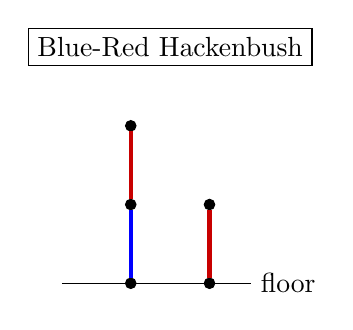
\begin{tikzpicture}
	\node[draw] (title) at (1.5, 3) {Blue-Red Hackenbush};
	\node (p1) at (0,0) {};
	\node (p2) at (3,0) {floor};
	\begin{scope} [every node/.style={scale=0.4, circle, draw, fill=black}]
		\node (p3) at (1,0) {};
		\node (p4) at (1,1) {};
		\node (p5) at (1,2) {};
		\node (p6) at (2,0) {};
		\node (p7) at (2,1) {};
		\draw (p1) -- (p2);
		\begin{scope} [ultra thick]
			\draw[blue] (p3) -- (p4);
			\draw[red] (p4) -- (p5);
			\draw[red] (p6) -- (p7);
		\end{scope}
	\end{scope}
\end{tikzpicture}


In this game, a move is made by taking a single colored edge of the image and removing any edges that become disconnected from the floor. One player can only remove blue edges, and the other, red edges.

It is a common practice to assume that, unless specified otherwise, games will be played between the players \naming{Left (bLue)} and \naming{Right (Red)}.




% Theory
    \chapter{Numbers are games. The reals, the ordinals and many others}
    \epigraph{``And behold! When the numbers had been created for infinitely many days, the universe itself appeared. And the evening and the morning were the $\aleph^[\footnotemark^]$ day. And Conway looked over the rules he had made for numbers, and saw that they were very, very good. And he commanded them to be for signs, and series, and quotients, and root. Then there sprang up an infinite number less than infinity. And infinities of days brought forth multiple orders of infinities"}{Donald Ervin Knuth, Surreal Numbers \footnotemark}

\footnotetext[1]{In order to match the the cardinal number notation, it would be more precise to write $\aleph_0$. The text will use the book notation $\aleph$.}

\footnotetext{Excerpt of the book \textit{Surreal Numbers: how two ex-students turned on to pure mathematics and found total happiness} that precedes the moment the couple define a rule for addition of numbers.}


Conway, by counting the number of spare moves a player has in combinatorial games, unveiled a new way to discover numbers. It is clear at this point that although numbers are not enough to represent games, they are the building blocks of all games, including the non-numbers. Until this point, the text showed some instances of the zero and hinted at $1$ and $-1$, and the reader may also guess on how to build any integer in RB-Hackenbush and Domineering. This chapter shows that knowing that is no more than scratching the surface of surreal numbers.

For the first parts of this section a number \gam{x_1, x_2,\, $\ldots$}{y_1, y_2,\,$\ldots$} might be called like a real number: $2, 5, 100000, \frac{1}{3}, \sqrt{10}, \pi$, but there is no reason believe this equality yet. There is also no reason to believe that $1 < 3$ or that $1 + 1 = 2$ yet. Up until this point, numbers are labels to games that trivially translated the number of spare moves a player has. However, first a few more numbers will be labeled and only then the operations and comparisons are defined.


\subsection*{Numbers Generated in Finite Steps}

It is known that \Gm{} =
\begin{tikzpicture}
	\draw[] (0.3,-0.3) rectangle ++(0.3,0.3);
	\draw[] (0,-0.3) rectangle ++(0.3,0.3);
\end{tikzpicture} = \gam{}{\gam{}{}} = \gam{}{0} and \Gm{} was labeled $-1$.
What would be a good label for \Hm = 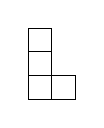
\begin{tikzpicture}
\draw[] (0.3,-0.3) rectangle ++(0.3,0.3);
\draw[] (0,-0.3) rectangle ++(0.3,0.3);
\draw[] (0,0) rectangle ++(0.3,0.3);
\draw[] (0,0.3) rectangle ++(0.3,0.3);
\end{tikzpicture}, given that it must be meaningful like described previously?\\ If it were to be labeled by a real number, which one should it be?

It is possible to find out a candidate by calculating \Gm{ + \Hm + \Hm}. To do that, one would usually find the game tree of 
\Gm{ + \Hm + \Hm} = 
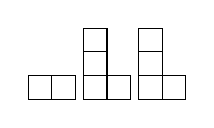
\begin{tikzpicture}
	\draw[] (-0.4,-0.3) rectangle ++(0.3,0.3);
	\draw[] (-0.7,-0.3) rectangle ++(0.3,0.3);
	\draw[] (0.3,-0.3) rectangle ++(0.3,0.3);
	\draw[] (0,-0.3) rectangle ++(0.3,0.3);
	\draw[] (0,0) rectangle ++(0.3,0.3);
	\draw[] (0,0.3) rectangle ++(0.3,0.3);
	\draw[] (1,-0.3) rectangle ++(0.3,0.3);
	\draw[] (0.7,-0.3) rectangle ++(0.3,0.3);
	\draw[] (0.7,0) rectangle ++(0.3,0.3);
	\draw[] (0.7,0.3) rectangle ++(0.3,0.3);
\end{tikzpicture}, and fill the known values bottom-up. However, it is simpler in this case. \Gm{ + 2\Hm = 0}, because whoever starts loses. Because \Gm{= -1}, a good label for \Hm is~$\frac{1}{2}$. Therefore:

$$H = \gam{{-}1, 0}{1} = \gam{0}{1} = \frac{1}{2}$$

 The second equality is true because Left would not move to $-1$ since it is a strictly worse move than moving the game to $0$. It might not seem natural for a player to be half a move up in a game, if he/she always plays one move at a time, but if it is desired that $\frac{1}{2} + \frac{1}{2} = 1$, that label makes sense for addition. It might be valuable to reiterate that \Hm is definitely positive because left wins no matter who starts, but $H < 1$, as Left does not have any spare moves, because $\Hm + \Gm = \Hm - 1 < 0$.

As one gets used to this kind of reasoning, it becomes clear that analyzing the game \gam{1}{} is the same as analyzing the game 
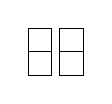
\begin{tikzpicture}
	\draw[] (0.3,-0.3) rectangle ++(0.3,0.3);
	\draw[] (0.3,0) rectangle ++(0.3,0.3);
	\draw[] (-0.1,0) rectangle ++(0.3,0.3);
	\draw[] (-0.1,-0.3) rectangle ++(0.3,0.3);
\end{tikzpicture}, but the former is not reliant on a specific ruleset. Rather, any combinatorial game has an instance equal to \gam{1}{}. However, the rules used to calculate the value of \Gm{=\gam{X}{Y}}, which are presented in the remaining of this section, help understand it better. The first practical rule in this text is finding the value of \gam{n}{} and \gam{}{{-}n}, for any natural number $n$.

Since 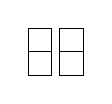
\begin{tikzpicture}
	\draw[] (0.3,-0.3) rectangle ++(0.3,0.3);
	\draw[] (0.3,0) rectangle ++(0.3,0.3);
	\draw[] (-0.1,0) rectangle ++(0.3,0.3);
	\draw[] (-0.1,-0.3) rectangle ++(0.3,0.3);
\end{tikzpicture} $= \gam{1}{}$, is it correct to assume that
$\underbrace{
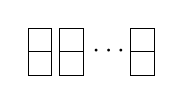
\begin{tikzpicture}
	\draw[] (1.2,-0.3) rectangle ++(0.3,0.3);
	\draw[] (1.2,0) rectangle ++(0.3,0.3);
	\draw[] (-0.1,0) rectangle ++(0.3,0.3);
	\draw[] (-0.1,-0.3) rectangle ++(0.3,0.3);
	\draw[] (0.3,0) rectangle ++(0.3,0.3);
	\draw[] (0.3,-0.3) rectangle ++(0.3,0.3);
	\node at (0.95, 0) {$\cdots$};
\end{tikzpicture}}_{n+1} = \gam{n}{}$? Yes, it is correct and the recursive nature of combinatorial games tell why. A $2\times 1$ board is equal to $1$ since Left has a move to spare. Therefore, two $2\times 1$ boards is equal to~$2$ since Left has a move to spare before reaching $1$. It is simple enough to visualize it in domineering boards. The fact is it should be simple to vizualise it in any combinatorial game. For any integer $k$, the game \gam{k}{} has the same value of the sum $\gam{k-1}{}+1$ if Left's best option $k$ is positive. If Left's best option is zero, then the game is equal to $1$, as already shown. If Left's best option is negative the result is zero, because Right cannot play, and  Left's move would result in the game $k$, which is negative, showing that whoever starts loses.  

In the case $k$ is positive, the addition $\gam{k-1}{} + 1$ was used. The notation is not the one used before, but it is possible replace $1$ with \gam{0}{}, as seen before. $\gam{k-1}{} + \gam{0}{}$ is an instance of addition described in the previous chapter. 

\begin{align*}
	\gam{k-1}{} + \gam{0}{} &\overset{def}{=} \gam{\gam{k-2}{} + \gam{0}{}, \gam{k-1}{} + \gam{}{}}{}\\
	&= \gam{\gam{k-2}{} + \gam{0}{}, \gam{k-1}{}}{}\\
	&\overset{def}{=} \gam{\gam{\gam{k-3}{} + \gam{0}{}}{}, \gam{\gam{k-2}{} + \gam{}{}}{}, \gam{\gam{k-2}{}}{}}{}\\
	&=\gam{\gam{\gam{k-3}{} + \gam{0}{}}{}, \gam{\gam{k-2}{}}{}, \gam{\gam{k-2}{}}{}}{}\\
	&=\gam{\gam{\gam{k-3}{} + \gam{0}{}}{}, \gam{\gam{k-2}{}}{}}{}\\
	&\overset{def}{\ldots}\\
	&=\underbrace{\{\{\ldots\{\{}_{k+1}\underbrace{\,|\,\}\,|\,\}\ldots\}\,|\,\}}_{k+1}\\
	&=\underbrace{\{\{\ldots\{\{}_{k} 0 \underbrace{\,|\,\}\,|\,\}\ldots\}\,|\,\}}_{k}\\
	&=\gam{k}{} = k + 1
\end{align*}

Every point discussed for \gam{X}{} is valid for \gam{}{Y}, through a similar argument. Up to this point, the integers and $\pm \frac{1}{2}$ are defined. The remaining numbers fall into three categories: the dyadic rationals - numbers of the form $\frac{a}{2^k}$, the numbers created in exactly infinite, $\aleph$, amount of steps, and the ones generated after more than infinite amount of steps. Of course the integers and $\frac{1}{2}$ fall into the first category.

In the case of $\Gm{} = \frac{1}{2} = \gam{0}{1}$, it is true that $G^L < G < G^R$. Is that always true? That is restricted for numbers, since in non-numbers \Gm{^R > G^L}. If Left makes a move from $G$ to $G^L$, is it true that Left has fewer spare moves in $G^L$ than in $G$? Before, as a side note, it was said that all possible RB-Hackenbush games are numbers, and the reason may help explain that it is true.

Suppose a game \Gm{ = \gam{X}{Y}} in which for all $x$ in $X$, $x$  is a number and for all $y$ in $Y$, $y$ is a number. Assume that $x_0$ in $X$ and $y_0$ in $Y$ are best moves for Left and Right respectively. If \Gm{} is not a number, than $x_0 \ge y_0$. Now consider \Hm an instance of RB-Hackenbush. A move in \Hm corresponds to removing a colored edge from a tree and all the edges that become disconnected to the floor. Assume again for \Hm that $x_0$ and $y_0$ are edges correspondent to the best moves for Left and Right respectively. That means that $x_0$ is similar to  
\begin{tikzpicture}
	\draw[blue, very thick] (0,0) -- (0,0.5);
	\node at (0, 0.9) {$\vdots$};
	\node at (-0.3, 0.9) {$\ddots$};
	\node at (0.3, 0.9) {\reflectbox{$\ddots$}};
\end{tikzpicture} and $y_0$ is similar to 
\begin{tikzpicture}
	\draw[red, dash pattern=on 3pt off 0.8pt, very thick] (0,0) -- (0,0.5);
	\node at (0, 0.9) {$\vdots$};
	\node at (-0.3, 0.9) {$\ddots$};
	\node at (0.3, 0.9) {\reflectbox{$\ddots$}};
\end{tikzpicture}. Is it possible that $G^{x_i} \ge G^{y_j}$?

Consider the game built by connecting $x_0$ to the floor. The game is definitely positive, as Left wins no matter who starts. If Right starts, he/she may have an available move in a edge above the one connected to the floor. Whether it is Left playing second or first, he/she may simply remove the blue edge connected to the floor, then Right has no moves remaining and loses the game. An analogous argument shows that $y_0$ in negative. Since $x_0$ is positive, the game $\Hm^{x_0}$ resulting from removing this positive branch is less positive, or more negative, than \Hm. The same way, $\Hm^{y_0}$ is more positive or less negative that \Hm. This fact, in turn, means that \Hm is a number.

Other phrasing for ``all RB-Hackenbush games are numbers" is ``it is not possible to make a move that improves your position in  RB-Hackenbush", or, ``Left cannot make a movement that increases the value of \Gm{}". Visualizing it brings the general idea why, in numbers, $G^L < G < G^R$. A more general approach is to consider, by induction, that $\Gm{^{LL}} < \Gm{^L} < \Gm{^{LR}}$ and $\Gm{^{RL}} < \Gm{^R} < \Gm{^{RR}}$. \Gm{^{LL}} translates to any possible Left move in \Gm{^L} and the others are defined similarly.

Consider the sum $\Gm{} - \Gm{^L}$. Before proceeding, the subtraction in this field means adding the negation. The negation of \gam{X}{Y} is \gam{-Y}{-X}. A good way to think of negation of a game \Gm{} as the same game \Gm{}, but with roles reversed. In the case of RB-Hackenbush for example, in ${-}\Gm{^L}$, Left plays the red edges. If Left starts, he/she can move to $\Gm{^L} - \Gm{^L} = 0$ and win the game. If Right starts, the game may be move to $\Gm{^R} - \Gm{^L}$ or $\Gm{} - \Gm{^{LR}}$. In the first case, it is clear that $\Gm{^R} - \Gm{^L} > 0$ because, from the definition of numbers, \Gm{^R} $>$ \Gm{^L}.
In the second case Left can move to $\Gm{^L} - \Gm{^{LR}}$, which is positive due to the induction hypothesis. Therefore, regardless who starts in $\Gm{} - \Gm{^L}$, Left wins, so the game is positive, meaning \Gm{>\Gm{^L}}. A similar argument shows that \Gm{<\Gm{^R}}.

Knowing this, however, is not enough to find the value of G. If $G = \{3 | 10\}$, it is clear that $3 < G < 10$ but what is the value of G? The simpler number that fits this interval, 4. What is called simpler is the minimal-birthday number that fits the interval. The word birthday comes from the initial analogy used to describe the creation of all the numbers. Before visiting the birthday tree and finishing explaining the simplicity principle, it is necessary to visit the definition of the comparison $\leq$.

Just like the definition of addition, the comparison is also done using game trees so it is the same for numbers and non-numbers. Consider the games \Gm{} and \Hm. \Gm{\leq \Hm} if they are equal or \Hm is more positive than \Gm{}. This condition is met if $\Hm > G^L$ and \Gm{<H^R}. These restrictions enforce that \Gm{=\gam{G^L}{G^R, H^R}} and $\Hm = \gam{G^L,H^L}{H^R}$, which guarantee the desired relation.

The birthday tree is the name given to the hierarchical structure that contains the definition of all surreal numbers. The tree is composed of layers, called generations, and each layer is a set of all the numbers formable with the available symbols. The zeroth generation is simply the set $\{0\} = \{\gam{}{}\}$. The first generation is the set $\{{-}1,0,1\}=$ \{\gam{}{0}, \gam{}{}, \gam{0}{}\}. The second is $\{-2,-1,\frac{-1}{2},0,\frac{1}{2},1,2\}$ and is equal to $\{\gam{}{{-}1},\gam{}{0},\gam{{-}1}{0},\gam{}{},\gam{0}{1}\gam{0}{},\gam{1}{}\}$. $0$ is called a zeroth generation number and $1$ and ${-}1$ are first generation numbers.

An important aspect of the generations is that, although labeling is not defined yet, they are fully ordered. Ordering is necessary for the simplicity rule because, as said before, \Gm{^L < \Gm{} < \Gm{^R}}. In order to find the value of \Gm{}, it is necessary to find a generation that contains both \Gm{^L} and \Gm{^R}, order it using the previously defined $\leq$ operation and find the oldest number lying strictly between \Gm{^L} and \Gm{^R}.

It is possible, however, to find cases where there are no numbers between \Gm{^L} and \Gm{^R}. In these case, one could look for a fitting number in the next generation. Another way to solve this is to notice that this cases occur if and only if both options are from the same generations and are neighbors in that generation. This condition implies that \Gm{^L = \frac{p}{2^q}} and \Gm{^R = \frac{p+1}{2^q}}. In this cases, the number in the next generation that lies strictly between them is the number \Gm{} and this number is labeled $\frac{2p + 1}{2^{q+1}}$.

The rules and definitions up until this point add up to:

\begin{center}
\Gm{ =} 
$
\begin{cases}
	0, &\text{if } G^L < 0 < G^R\\
	n+1, &\text{if } \Gm{= \gam{n}{}}\\
	-n-1, &\text{if } \Gm{= \gam{}{{-}n}}\\
	\frac{2p + 1}{2^{q+1}}, &\text{if } \Gm{= \gam{\frac{p}{2^q}}{ \frac{p+1}{2^q}}}\\
	\text{search the tree} &\text{otherwise}
\end{cases}
$
\end{center}

\vspace{0.6em}Some examples are $\frac{1}{4} =$ \gam{\frac{1}{10}}{\frac{3}{10}}, $\frac{1}{8} =$ \gam{0}{\frac{1}{4}}, $10 =$ \gam{9}{}, $1 =$ \gam{\frac{1}{2}}{}. The first and last examples require some manipulation as they would require a search on the birthday tree, as described previously. This would be a problem because both options of the first example would require an infinite number of generations to be created. However, since the embedded real numbers ought to be ordered the same and since surreals numbers are generated successively, the first number that fits the interval is the simplest that fits. Since $\frac{1}{10} < \frac{1}{4} < \frac{3}{10}$ and no older number older fits, the equality stands.

The remaining problematic example is $1 =$ \gam{\frac{1}{2}}{}. Consider the games, which happen to be numbers, \Gm{= \gam{0}{}} and $H = \gam{\frac{1}{2}}{}$. $G = 1$, directly from the simplicity rules. It is said that $H = 1$, but that is not a direct implication. It is possible, however, to show $G \leq H \leq G$. $H \leq G$, because $0.5$ is the only Left option of $H$, there are no Right options in $G$ and $0.5 < G = 1$. $G \leq H$, because $0$ is the only Left option of $G$, there are no Right options in $H$ and $0 < H$. The last inequality, $0 < H$, is true because in the game $H$, Left wins no matter who starts, and this means the game is positive.

It is possible to think of many other cases that require other manipulations to fall into the precisely defined rules. The reality is that the first four rules and the $\leq$ comparison are enough to label all the numbers. The fuzzy notion of simplicity brought in the last few paragraphs helps finding and understanding the reason for labels given but it is not necessary. The `Simplicity Rules' are actually just the first four rules.

\begin{center}
	\Gm{ =} 
	$
	\begin{cases}
		0, &\text{if } G^L < 0 < G^R\\
		n+1, &\text{if } \Gm{= \gam{n}{}}\\
		-n-1, &\text{if } \Gm{= \gam{}{{-}n}}\\
		\frac{2p + 1}{2^{q+1}}, &\text{if } \Gm{= \gam{\frac{p}{2^q}}{ \frac{p+1}{2^q}}}
	\end{cases}
	$
\end{center}

\subsection*{Numbers generated after infinite steps}

The formula above only allows \Gm{} to have an infinite amount of values, but the dimension of this infinity might not approach the stated in the beginning of the section yet. The remaining numbers are hidden in the end of infinite games. Infinite games, in this section, indicate board sizes that infinite, not infinite play, because, as explained before, this text only deals with short games. 

\begin{figure} [!ht]
\begin{center}
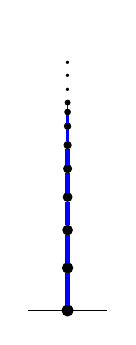
\begin{tikzpicture}
	\begin{scope} [every node/.style={scale=0.3, style=circle, draw, fill=black}]
		\node [scale=1.4] (1) at (0, -1.80){};
		\node [scale=1.3] (2) at (0, -1.26){};
		\node [scale=1.2] (3) at (0, -0.78){};
		\node [scale=1.1] (4) at (0, -0.36){};
		\node [scale=1]   (5) at (0, 0)      {};
		\node [scale=0.9] (6) at (0, 0.3)  {};
		\node [scale=0.8] (7) at (0, 0.54) {};
		\node [scale=0.7] (8) at (0, 0.72) {};
		\node [scale=0.6] (9) at (0, 0.84) {};
		\node [scale=0.2, fill=white, draw=none] at (0, 1.1) {$\vdots$};
	\end{scope}
	\draw (-0.5,-1.80) -- (0.5, -1.80);
	\draw[blue, ultra thick] (1)--(2);
	\draw[blue, ultra thick] (2)--(3);
	\draw[blue, ultra thick] (3)--(4);
	\draw[blue, ultra thick] (4)--(5);
	\draw[blue, ultra thick] (5)--(6);
	\draw[blue, thick] (6)--(7);
	\draw[blue, thick] (7)--(8);
	\draw[blue] (8)--(9);
	\node[scale=1.5] at (0, 1.3) {\scriptsize$\vdots$};
\end{tikzpicture}
\end{center}
\end{figure}

In the game above, Left has an infinite number of possible moves, but his/her move always leads to an integer. What is the value of this game? \gam{1,2,...}{}, the one more than the largest natural number. This number has been baptized much earlier in mathematics. It was called $\omega$, the first ordinal number, and the label is kept in the surreal numbers. It might not be as straight forward as finitely generated numbers, but the principle to calculate the value is the same.

For any finite number of red edges in \Gm{}, if you add the game above to \Gm{}, the result will be positive. However, it is also very simple to verify that $\omega$ is by far not the largest possible advantage. One simple  example for that is the following section.

$\omega$ is one of numbers generated in the $\aleph$ generation. Another is the number \gam{0}{\frac{1}{1}, \frac{1}{2}, \ldots}, labeled $\epsilon$. This number is positive, as Left wins no matter who starts, but it is smaller than any positive real number. A game with value $\epsilon$ may be simply the game of RB-Hackenbush starting with a blue edge and following with an infinite number of red edges.

These numbers are special in the sense that they are the first non-real numbers to show up, but they are not the only non-reals and they are not the only members of their generation. The integers and dyadic rationals show up in earlier generations, but the remaining reals all show up in the $\aleph$ generation. Chapter 5 will develop this topic a little further but, in general, it is not paramount to the topic of temperature.

\subsection*{Numbers generated after more than infinite steps}

\begin{figure} [!ht]
\begin{center}
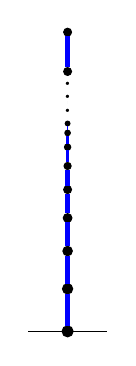
\begin{tikzpicture}
	\begin{scope} [every node/.style={scale=0.3, style=circle, draw, fill=black}]
		\node [scale=1.4] (1) at (0, -1.80){};
		\node [scale=1.3] (2) at (0, -1.26){};
		\node [scale=1.2] (3) at (0, -0.78){};
		\node [scale=1.1] (4) at (0, -0.36){};
		\node [scale=1]   (5) at (0, 0)      {};
		\node [scale=0.9] (6) at (0, 0.3)  {};
		\node [scale=0.8] (7) at (0, 0.54) {};
		\node [scale=0.7] (8) at (0, 0.72) {};
		\node [scale=0.6] (9) at (0, 0.84) {};
		\node [scale=0.2, fill=white, draw=none] at (0, 1.1) {$\vdots$};
		\node [scale=1] (10) at (0, 1.5) {};
		\node [scale=1] (11) at (0, 2) {};
	\end{scope}
	\draw (-0.5,-1.80) -- (0.5, -1.80);
	\draw[blue, ultra thick] (1)--(2);
	\draw[blue, ultra thick] (2)--(3);
	\draw[blue, ultra thick] (3)--(4);
	\draw[blue, ultra thick] (4)--(5);
	\draw[blue, ultra thick] (5)--(6);
	\draw[blue, thick] (6)--(7);
	\draw[blue, thick] (7)--(8);
	\draw[blue] (8)--(9);
	\node[scale=1.5] at (0, 1.3) {\scriptsize$\vdots$};
	\draw[blue, ultra thick] (10)--(11);
\end{tikzpicture}
\end{center}
\end{figure}

The game above is an infinite stack of blue edges with another one on the top. One could wrongly argue that this additional edge on the top is simply part of the infinite stack. This is a wrong argument because this additional edge on the top allows Left to move to $\omega$, and therefore, has the value of $\omega+1$, making the games different. The reason why in this case you can move to $\omega$ is that you can move on the top-most edge, while before, there was no top-most edge. This detail is paramount to understanding the statement found on the epigraph of this section.

A hypothetical John Horton Conway wrote the paragraph found on the epigraph near a cave close to the edge of the Indian Ocean, where a couple of future mathematicians went to find themselves. The words attributed to Conway by Knuth say that in the $\aleph$th day the universe appeared. That is because Knuth realizes that in that specific days all real numbers are generated.

However, again, accordingly to the hypothetical Conway, days kept passing by and more numbers were generated. The number $\omega+1$ is one of the infinitely many surreal numbers that are not real numbers. However, this is not the end of the story. In fact, even considering that $\omega + \omega + ...$ and $\omega^\omega$ are also generated in the same format, the important part might again be missed. That is because looking at large numbers is not the only way forward.

Now that $\epsilon$ is a known members of the $\aleph$ generation, it is possible to make numbers like \gam{0}{\epsilon} and \gam{-\epsilon}{0} and also games like \gam{1}{1 + \epsilon} and \gam{1-\epsilon}{1}. As the generations keep getting created it is easy to see that there are infinite numbers that are positive but less than any positive real number. In fact if taking the example around 1, it is possible to notice that between any two real numbers there are infinite non-real numbers. These non-real numbers are called infinitesimals.

There are still more non-real number that are not infinitesimals nor cardinals. A good example is the number $\sqrt{\omega} = \gam{1,2,3,\ldots}{\omega, \frac{\omega}{2},\frac{\omega}{4},\ldots}$. To verify that the label $\sqrt{\omega}$ is proper one would need to learn the definition of multiplication and verify that $\sqrt{\omega} \cdot \sqrt{\omega} = \omega$. As this text makes no use of multiplication this is not going to be verified. This example serves only to contribute to the point that there are truly many numbers originating from the simplicity rules.

\subsection*{The Surreal Numbers}

This text presents only few characteristics of the surreal numbers as they are not the focus. It is also not necessary to know every algebraic property of numbers to go forward with the study of temperature this text focus on. However, it so happens that with very few construction rules, the numbers contain all the reals, the ordinals, the infinitesimals numbers.

Because of its extremely simple definition and big expressiveness, it is an extremely interesting topic. The idea that the number of spare moves a player has might not be a real number might not be confusing, but it should be somewhat hard to accept. It is true that this fact is based on the construction Conway made and it is not necessarily true for all ways to analyze games, but the straight forward way of using game trees to build numbers lead to this characteristic.

Because the creation/discovery of surreals is very recent, it definitely makes people apprehensive as it is not clear if its properties are good or bad. The mathematician Phillip Ehrlich is an eloquent participant in this discussion. He makes the point that the surreals do not have an intrinsic problem and that they show an unifying nature between paths in mathematics. In one of his papers, Ehrlich proposes that, while the real numbers form, on his words, an arithmetic continuum, the surreals form the absolute arithmetic continuum\cite{7}.

However, it is still a problem converting the domain of typical studies, such as calculus, from the reals to the surreals. Integrals of functions in the surreals are particularly hard to define. In the 2015 revision of their paper \cite{8}, Salzedo and Swaminathan made important contributions. For reference, they proved the intermediate value theorem in \textbf{No}, how the class of all surreal numbers is called. However, for example, they used a definition of integration that, although solving a problem with previous definitions, they make it clear that other problems persist.

As the same authors point-out: ``The `Conway-Norton'\footnote{In ONAG 2nd edition page 228, Conway  tells that Norton's definition of integrals do not have desired properties.}
integral failed to have standard properties of real integration, however, such as translation
invariance: $\int_a^bf(x)dx = \int_{a-t}^{b-t}f(x+t)dx$, for any surreal function f and $a,b,t\in$ \textbf{No}. While Fornasiero fixed this issue \cite{9}, the new integral, like its predecessor, yields
$exp(\omega)$ instead of the desired $exp(\omega)-1$ for $\int_0^{\omega}exp(x)dx$". In the ``Open Questions" section of  the paper, the authors tell that there are still problems with their definition, meaning that the conversion of domains in integral studies is not completed, at least by 2015.

While many questions remain open, however, it is still possible to work with a subset of the surreals that only contain the reals for example. The remaining of the text does not require profound knowledge of anything that is not mentioned in regards to numbers.










    
% Data
    \chapter{Heating things up}
    
\definecolor{purple2}{RGB}{218,112,214}

This sections will provide new tools and ideas to analyze games and to do that, the same strategy of the previous section will be followed. Initially, the reader is presented with an intuitive idea and preliminary formulation of the problem. The first part contains many examples and its intent is to provide the reader enough to use the more mathematical heavy part to in fact gain advantage in any game played.

Now that enough is known about numbers, it is possible to work with non-numbers. The only known non-numbers at this point are the switches. But is knowing what they are enough to playing them? The game simpler cashing cheques will tell.

In this game there is a table with purple cheques. Each cheque has two numbers written on top, and, in each player's turn they will either pay one coin or cash a cheque that will grant him a number of coins equal to the correspondent associated integer. What is the best move for Left?

\begin{center}
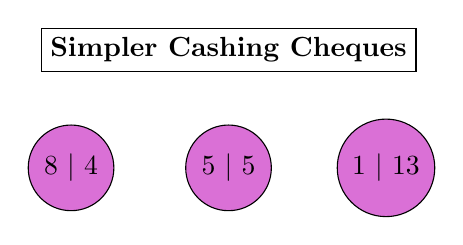
\begin{tikzpicture}
	\node[draw] (title) at (0,1.5) {\textbf{Simpler Cashing Cheques}};
	\begin{scope} [every node/.style={style=circle, draw, fill=purple2}]
		\node at (-2,0) {8 $|$ 4};
		\node at (0,0) {5 $|$ 5};
		\node at (2,0) {1 $|$ 13};
	\end{scope}
\end{tikzpicture}
\end{center}

Definitely the move is not paying, as Left can earn money in his turn. A good thing to grasp from this example is that you should never play in a number, paying a coin in this case, if there are non-numbers, cashing a purple cheque in this case. Should Left cash 8, 5 or 1? 1, of course. The reader is encouraged to play as Left and trying to find the best possible outcome, but the answer is playing the hottest switch. Although the game above is not a switch, it is a sum of switches, and, because of that can benefit of the simplified notation discussed earlier.

\begin{align*}
	G =& \left(\frac{8-4}{2} \pm \frac{8+4}{2}\right) + \left(\frac{5-5}{2} \pm \frac{5+5}{2}\right) + \left(\frac{1-13}{2} \pm \frac{1+13}{2}\right) \\
	  =& (2 \pm 6) + (0 \pm 5) + (-6 \pm 7)\\
	  =& -4 \pm 7 \pm 6 \pm 5
\end{align*}

If you analyze the result above, it becomes clear that Left must play on the rightmost component as, although it will not provide many coins, it will prevent right from cashing a huge amount. It is very possible to build scenarios where a player would even pay for cashing a cheque if that prevented the opponent from getting rich. Now that playing a simpler cashing cheques became easy, a more challenging task will rise. How to play Domineering well?

Adding a number with a temperature in a simplified position, like the expression above, should be acceptable by anyone following up to this point. Following, in the other hand, numbers will be added together with non-numbers just like number are added together and this might cause confusion. However, understanding that this sum is possible and intuitive is simple.

Playing a sum of games is just like playing a game with a set of independent rulesets and components. \begin{center}
	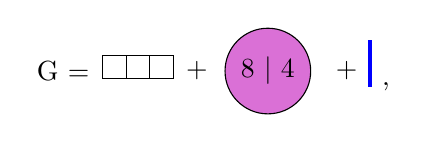
\begin{tikzpicture}
		\node at (-0.5,0.1) {G =};
		\draw[] (0,0) rectangle ++(0.3,0.3);
		\draw[] (0.3,0) rectangle ++(0.3,0.3);
		\draw[] (0.6,0) rectangle ++(0.3,0.3);
		\node at (1.2,0.1) {$+$};
		\node[style=circle, draw, fill=purple2] at (2.1,0.1) {8 $|$ 4};
		\node at (3.1,0.1) {$+$};
		\draw[color=blue, ultra thick] (3.4, -0.1) -- (3.4, 0.5);
		\node[] at(3.6, -0.1) {,};
		\end{tikzpicture}
\end{center}
for example, is a game where each player makes a move\footnote{There are other ways of playing G that will not be discussed} in any of the components and loses if cannot make a move. In other words, \Gm{} is a game like every other, except for the more complex ruleset.

The result of this sum is obvious if all components are also numbers or switches. In the case of playing numbers and general non-numbers, sensible players will always play in non-numbers first. With this in mind other facts become clear. The first is that the temperature of a non-number added to a number is unaltered.

The second is that such a sum is actually a sum of non-numbers, added together with a number after they cool out. The sum of general non-numbers is thoroughly discussed in the remaining of the chapter, however, it worth noticing what the goal of this discussion is.

By the end of this section it will be thought how to convert any game in a 2D graphic composed of two \todo{curves} that collapse to one line at some point, whose axes is number x cooling factor. The purpose of all this is that if the ending point falls in the positive side, Left gets an advantage, and if it falls in the positive, right does.

To build this graphic one is required to traverse the game tree, so the effort may seem fruitless as the game tree itself provides the winning strategy by itself. However, in cases where the game tree resulting from the sum of games is too large or expensive for a computer to run, there is a good strategy to playing this sum without knowing the complete game tree. In order to build the thermograph and play the \defi{thermostrat}\footnote{This text will not present the thermostrat} correctly, there are a lot of minor concepts not discussed yet.

Other than the bias, playing a game like Domineering well involves the concepts of \defi{Left/Right stops}, \defi{toenail}, \defi{ambient temperature}, \defi{freezing point}, \defi{cooling}, \defi{heating} and a few others. To put all that together and provide a clear visualization of the best strategy, the thermograph.

\begin{center}
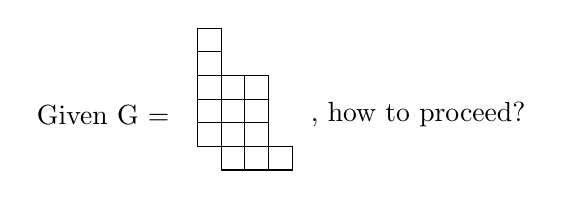
\begin{tikzpicture}
	\node at (-1.5,0.1) {Given G =};
	\draw[] (0,-0.6) rectangle ++(0.3,0.3);
	\draw[] (0.3,-0.6) rectangle ++(0.3,0.3);
	\draw[] (0.6,-0.6) rectangle ++(0.3,0.3);
	\draw[] (-0.3,-0.3) rectangle ++(0.3,0.3);
	\draw[] (0,-0.3) rectangle ++(0.3,0.3);
	\draw[] (0.3,-0.3) rectangle ++(0.3,0.3);
	\draw[] (-0.3,0) rectangle ++(0.3,0.3);
	\draw[] (0,0) rectangle ++(0.3,0.3);
	\draw[] (0.3,0) rectangle ++(0.3,0.3);
	\draw[] (-0.3,0.3) rectangle ++(0.3,0.3);
	\draw[] (0,0.3) rectangle ++(0.3,0.3);
	\draw[] (0.3,0.3) rectangle ++(0.3,0.3);
	\draw[] (-0.3,0.6) rectangle ++(0.3,0.3);
	\draw[] (-0.3,0.9) rectangle ++(0.3,0.3);
	\node at (2.5,0.1) {, how to proceed?};
\end{tikzpicture}
\end{center}

\begin{center}
	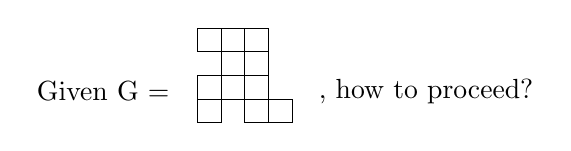
\begin{tikzpicture}
		\node at (-1.2,0.1) {Given G =};...
		\draw[] (0.6,-0.3) rectangle ++(0.3,0.3);
		\draw[] (0.9,-0.3) rectangle ++(0.3,0.3);
		\draw[] (0,-0.3) rectangle ++(0.3,0.3);
		\draw[] (0,0) rectangle ++(0.3,0.3);
		\draw[] (0.3,0) rectangle ++(0.3,0.3);
		\draw[] (0.6,0) rectangle ++(0.3,0.3);
		\draw[] (0.3,0.3) rectangle ++(0.3,0.3);
		\draw[] (0.6,0.3) rectangle ++(0.3,0.3);
		\draw[] (0,0.6) rectangle ++(0.3,0.3);
		\draw[] (0.3,0.6) rectangle ++(0.3,0.3);
		\draw[] (0.6,0.6) rectangle ++(0.3,0.3);
		\node at (2.9,0.1) {, how to proceed?};
	\end{tikzpicture}
\end{center}

G is definitely not a switch nor a sum of switches. It is possible to say the temperature in G is going to stay high for quite some time, because hotness is a term used to define the importance of the next move. A good place to start is writing out the game tree and building a temperature graphic of how it builds up from simpler positions until the more complicated ones.

To decrease the confusion that builds up in complicated positions, there is the idea of a cooling factor. The non-number \Gm{} cooled by $t$ degrees is represented by \Gm{_t} and is defined by:
\begin{center}
	\Gm{_t} = \gam{\Gm{^L_t} - t}{\Gm{^R_t} + t} $\forall t \leq t'$\\
	\Gm{_t} = x $\forall t > t'$\\
	Given $t'$ is the smallest cooling factor such\\
	that \Gm{_{t'}} is infinitesimally close to a number $x$,
\end{center}

The temperature $t(G)$ is equal to $t'$. Now that both axes are defined, some examples of thermographs:

\begin{tikzpicture}
	\begin{axis}
		[
		title = \Gm{=} \gam{3}{1},
		xmin=0.5,xmax=3.5, x dir=reverse, xtick={0, 1, 2, 3},
		ymax=3, ytick={0, 0.5, 1},
		axis x line*=none, axis y line*=none,
		axis line style={draw=none},
		y label style={rotate=-90,at={(current axis.north west)}, right=5mm},
		ylabel = \textbf{t}
		]
		\addplot[black] coordinates {
		(0.5,0)(3.5,0)
		};
		\addplot[black, very thick] coordinates {
		(0.9,-0.1)(2,1)
		};
		\addplot[black, very thick] coordinates {
		(3.1,-0.1)(2,1)
		};
		\addplot[black,-{Latex[length=3mm]}, very thick] coordinates {
		(2,1)(2,2)
	};
	\end{axis}
	\begin{axis}
	[
	at={(0.5\linewidth,0)},
	title = \Gm{=} \gam{0}{{-}4},
	xmin=-4.5,xmax=0.5, x dir=reverse, xtick={-4, -2, 0},
	ymax=3, ytick={0, 1, 2},
	axis x line*=none, axis y line*=none,
	axis line style={draw=none},
	y label style={rotate=-90,at={(current axis.north west)}, right=5mm},
	ylabel = \textbf{t}
	]
	\addplot[black] coordinates {
		(0.5,0)(-4.5,0)
	};
	\addplot[black, very thick] coordinates {
		(-0.1,-0.1)(-2,2)
	};
	\addplot[black, very thick] coordinates {
		(-4.1,-0.1)(-2,2)
	};
	\addplot[black,-{Latex[length=3mm]}, very thick] coordinates {
		(-2,2)(-2,2.5)
	};
	\end{axis}
	\begin{axis}
	[
	at={(0,-330)},
	title = \Gm{=} \gam{0}{0},
	xmin=-0.5,xmax=0.5, x dir=reverse, xtick={0},
	ymax=2, ytick={0, 1},
	axis x line*=none, axis y line*=none,
	axis line style={draw=none},
	y label style={rotate=-90,at={(current axis.north west)}, right=5mm},
	ylabel = \textbf{t}
	]
	\addplot[black] coordinates {
		(-0.5,0)(0.5,0)
	};
	\addplot[black, very thick] coordinates {
		(-0.1,-0.1)(0,0)
	};
	\addplot[black, very thick] coordinates {
		(0.1,-0.1)(0,0)
	};
	\addplot[black,-{Latex[length=3mm]}, very thick] coordinates {
		(0,0)(0,1.5)
	};
	\end{axis}
	\begin{axis}
	[
	at={(0.5\linewidth,-330)},
	title = \Gm{=} \gam{0}{\gam{0}{0}},
	xmin=-0.5,xmax=0.5, x dir=reverse, xtick={0},
	ymax=2, ytick={0, 1},
	axis x line*=none, axis y line*=none,
	axis line style={draw=none},
	y label style={rotate=-90,at={(current axis.north west)}, right=5mm},
	ylabel = \textbf{t}
	]
	\addplot[black] coordinates {
		(-0.5,0)(0.5,0)
	};
	\addplot[black, very thick] coordinates {
		(0,-0.1)(0,0)
	};
	\addplot[black, very thick] coordinates {
		(0.1,-0.1)(0,0)
	};
	\addplot[black,-{Latex[length=3mm]}, very thick] coordinates {
		(0,0)(0,1.5)
	};
	\end{axis}
\end{tikzpicture}


Some characteristics might be immediately apparent. The first is that the x-axis is reversed. The reason for that is to keep Right's movements to the right and Left's to the left. The second characteristic may be that all the thermographs end with a vertical \defi{mast}. The mast begins at $t'$ and indicates that \Gm{} is a number from that point forward. The last one is that the graphic continues past the $y=0$ line. It is worth noticing that the difference between the last two thermographs is below the $y=0$ line.

Toenails, the segments below the $y=0$ line, are important and may seem different, but they are actually simple extensions of the graphic. The reason for the last two toenails to be different is that cooling is applied to all the Left and Right alternatives, but in opposite directions. It is important to remember \hbox{\Gm{_t} = \gam{\Gm{^L_t} - t}{\Gm{^R_t} + t}}, because it explains the difference. Both Left's and the first Right's toenail came from cooling 0, but the second Right's toenail came from cooling \gam{0}{0}.

The next example, the second of non-switch hot games, shows how cooling $L$ and $R$ alternatives work.\\

\begin{figure}[H]
\begin{center}
	\scalebox{0.8}{
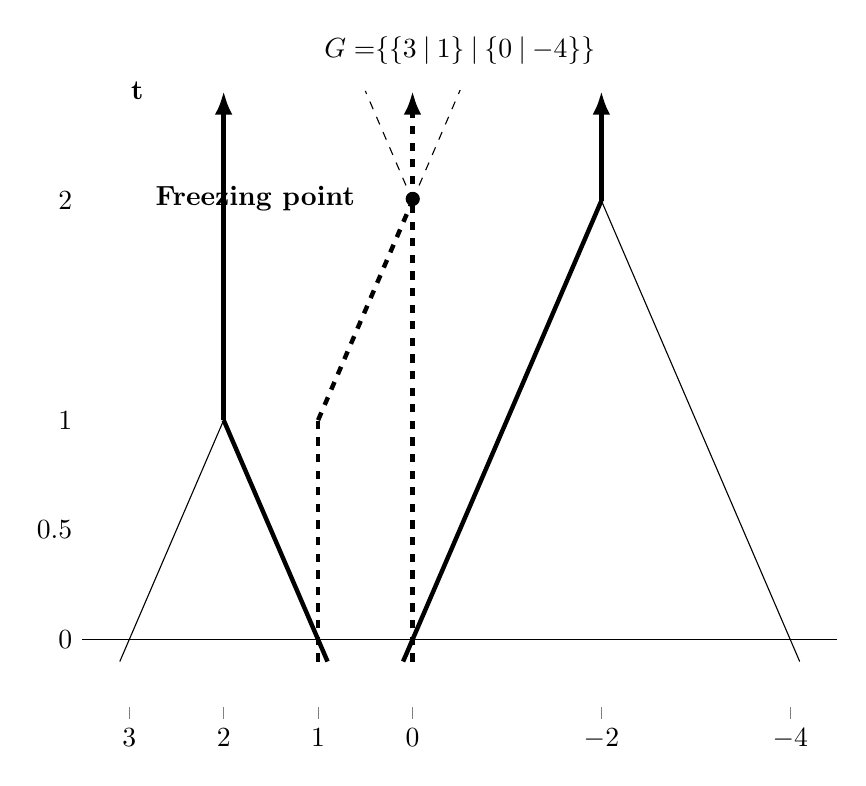
\begin{tikzpicture}
	\node[] at (2.2, 6.6) {\textbf{Freezing point}};
	\node[scale=0.5, circle, draw, fill=black] at (4.2, 6.6) {};
	\begin{axis}
		[
		title = \Gm{=}\gam{\gam{3}{1}}{\gam{0}{{-}4}},
		xmin=-4.5,xmax=3.5, x dir=reverse, xtick={-2, -4, 0, 1, 2, 3},
		ymax=2.5, ytick={0, 0.5, 1, 2},
		axis x line*=none, axis y line*=none,
		axis line style={draw=none},
		y label style={rotate=-90,at={(current axis.north west)}, right=5mm},
		ylabel = \textbf{t},
		scale=1.4
		]
		
		\addplot[black] coordinates {
			(-4.5,0)(3.5,0)
		};
		\addplot[ultra thick] coordinates {
			(0.9,-0.1)(2,1)
		};
		\addplot[black] coordinates {
			(3.1,-0.1)(2,1)
		};
		\addplot[-{Latex[length=3mm]}, ultra thick] coordinates {
			(2,1)(2,2.5)
		};
		\addplot[ultra thick] coordinates {
			(0.1,-0.1)(-2,2)
		};
		\addplot[] coordinates {
			(-4.1,-0.1)(-2,2)
		};
		\addplot[-{Latex[length=3mm]}, ultra thick] coordinates {
			(-2,2)(-2,2.5)
		};
		\addplot[black, dashed, ultra thick] coordinates {
			(1,-0.1)(1,1)
		};
		\addplot[black, dashed, ultra thick] coordinates {
			(0,-0.1)(0,2)
		};
		\addplot[black, dashed, ultra thick] coordinates {
			(1,1)(0,2)
		};
		\addplot[black, dashed] coordinates {
			(0,2)(-1,3)
		};
		\addplot[black, dashed] coordinates {
			(0,2)(0.5,2.5)
		};
		\addplot[black, dashed, ultra thick, -{Latex[length=3mm]}] coordinates {
			(0,2)(0,2.5)
		};
	\end{axis}
\end{tikzpicture}}
\end{center}
\caption{The dissection of a thermograph}
\end{figure}



In the example above, the thick dashed thermograph is the thermograph of G. The light dashed segments are illustrative extensions of the cooling of L and R. The bold lines were used to show what part of L and R are taken into consideration: Right's slant is used to build Left's slant and vice-versa. The reason for this is that after either player makes a move, it will be the opponent's turn to move, and, this way, the opposing slant is the important one.

It is also worth mentioning that a freezing point will always be reached after an equal amount of move by each player. In the example above, the freezing point is the same as the junction point where the right slant bends, but that is not always the case. Before visiting \todo{siegel}'s formulation of the problem, one that brings good notation and formalism, an example of a real scenario is due. In a fun game each player has more than one option for their moves and that has not been addressed yet.

What is the thermograph of the game \Gm{=}
	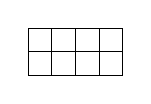
\begin{tikzpicture}
		\draw[] (0.6,-0.6) rectangle ++(0.3,0.3);
		\draw[] (0.3,-0.6) rectangle ++(0.3,0.3);
		\draw[] (0.9,-0.6) rectangle ++(0.3,0.3);
		\draw[] (0,-0.6) rectangle ++(0.3,0.3);
		\draw[] (0,-0.3) rectangle ++(0.3,0.3);
		\draw[] (0.3,-0.3) rectangle ++(0.3,0.3);
		\draw[] (0.6,-0.3) rectangle ++(0.3,0.3);
		\draw[] (0.9,-0.3) rectangle ++(0.3,0.3);
	\end{tikzpicture} ? 

\begin{figure} [!ht]
\begin{center}
\begin{tikzpicture}
	[
	sibling distance=150pt,
	level distance=100pt,
	level 1/.style={sibling distance=4cm},
	level 2/.style={sibling distance=1.7cm},
	every node/.style = {
	},
	every child/.style = {
		ultra thick
	}
	]

\node[draw] (title) at (0, 1) {Game Tree};

\node {
	\begin{tikzpicture}
		\draw[] (0.6,-0.6) rectangle ++(0.3,0.3);
		\draw[] (0.3,-0.6) rectangle ++(0.3,0.3);
		\draw[] (0.9,-0.6) rectangle ++(0.3,0.3);
		\draw[] (0,-0.6) rectangle ++(0.3,0.3);
		\draw[] (0,-0.3) rectangle ++(0.3,0.3);
		\draw[] (0.3,-0.3) rectangle ++(0.3,0.3);
		\draw[] (0.6,-0.3) rectangle ++(0.3,0.3);
		\draw[] (0.9,-0.3) rectangle ++(0.3,0.3);
	\end{tikzpicture}}
child[blue, level distance=80pt] {node[black] {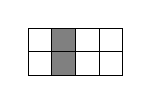
\begin{tikzpicture}
			\draw[] (0.6,-0.6) rectangle ++(0.3,0.3);
			\draw[fill=gray] (0.3,-0.6) rectangle ++(0.3,0.3);
			\draw[] (0.9,-0.6) rectangle ++(0.3,0.3);
			\draw[] (0,-0.6) rectangle ++(0.3,0.3);
			\draw[] (0,-0.3) rectangle ++(0.3,0.3);
			\draw[fill=gray] (0.3,-0.3) rectangle ++(0.3,0.3);
			\draw[] (0.6,-0.3) rectangle ++(0.3,0.3);
			\draw[] (0.9,-0.3) rectangle ++(0.3,0.3);
	\end{tikzpicture}}
	child[blue] {node[black] {\gam{1}{}}}
	child[blue] {node[black] {\gam{1}{{-}1}}}
	child[red, dashed] {node[black] {\gam{{-}1}{1}}}
}
child[blue] {node[black] {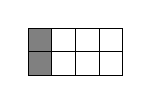
\begin{tikzpicture}
			\draw[] (0.6,-0.6) rectangle ++(0.3,0.3);
			\draw[] (0.3,-0.6) rectangle ++(0.3,0.3);
			\draw[] (0.9,-0.6) rectangle ++(0.3,0.3);
			\draw[fill=gray] (0,-0.6) rectangle ++(0.3,0.3);
			\draw[fill=gray] (0,-0.3) rectangle ++(0.3,0.3);
			\draw[] (0.3,-0.3) rectangle ++(0.3,0.3);
			\draw[] (0.6,-0.3) rectangle ++(0.3,0.3);
			\draw[] (0.9,-0.3) rectangle ++(0.3,0.3);
	\end{tikzpicture}}
	child[blue] {node[black] {\gam{1}{}}}
	child[blue] {node[black] {\gam{1}{{-}1}}}
	child[red, dashed] {node[black] {\gam{{-}1}{0,1}}}
}
child[red, dashed, level distance=80pt] {node[black, solid] { 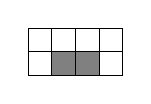
\begin{tikzpicture}
			\draw[fill=gray] (0.6,-0.6) rectangle ++(0.3,0.3);
			\draw[fill=gray] (0.3,-0.6) rectangle ++(0.3,0.3);
			\draw[] (0.9,-0.6) rectangle ++(0.3,0.3);
			\draw[] (0,-0.6) rectangle ++(0.3,0.3);
			\draw[] (0,-0.3) rectangle ++(0.3,0.3);
			\draw[] (0.3,-0.3) rectangle ++(0.3,0.3);
			\draw[] (0.6,-0.3) rectangle ++(0.3,0.3);
			\draw[] (0.9,-0.3) rectangle ++(0.3,0.3);
	\end{tikzpicture}}
	child[blue, solid] {node[black] {\gam{{-}1}{0, 1}}}
	child[red] {node[black] {\gam{1}{}}}
	child[red] {node[black] {\gam{0}{0}}}
}
child[red, dashed] {
	node[black, solid] { 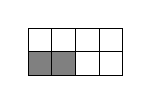
\begin{tikzpicture}
	\draw[] (0.6,-0.6) rectangle ++(0.3,0.3);
	\draw[fill=gray] (0.3,-0.6) rectangle ++(0.3,0.3);
	\draw[] (0.9,-0.6) rectangle ++(0.3,0.3);
	\draw[fill=gray] (0,-0.6) rectangle ++(0.3,0.3);
	\draw[] (0,-0.3) rectangle ++(0.3,0.3);
	\draw[] (0.3,-0.3) rectangle ++(0.3,0.3);
	\draw[] (0.6,-0.3) rectangle ++(0.3,0.3);
	\draw[] (0.9,-0.3) rectangle ++(0.3,0.3);
	\end{tikzpicture}}
		child[blue, solid] {node[black] {\gam{{-}1}{1}}}
		child[blue, solid] {node[black] {\gam{{-}1}{0,1}}}
		child[red] {node[black] {\gam{}{{-}1}}}
	}
;

\end{tikzpicture}
\end{center}
\end{figure}

\hspace{-1cm}
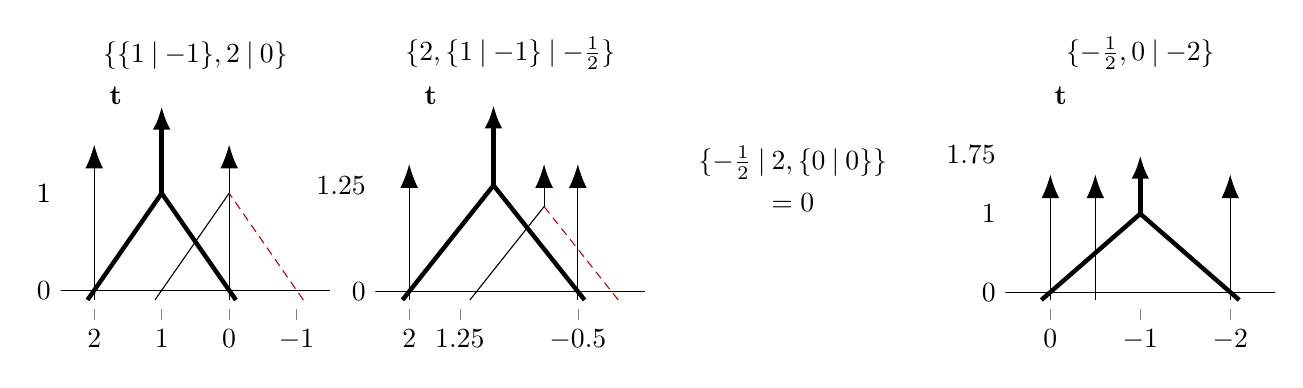
\begin{tikzpicture}
\begin{axis}
	[
		title = \gam{\gam{1}{{-}1},2}{0},
		xmin=-1.5,xmax=2.5, x dir=reverse, xtick={-1,0, 1, 2},
		ymax=2, ytick={0, 1, 1},
		scale=0.5,
		style thermograph
	]
	\addplot[] coordinates {(3.5,0)(-1.5,0)};
	\addplot[-{Latex[length=3mm]}] coordinates { (2,-0.1)(2,1.5)};
	\addplot[-{Latex[length=3mm]}] coordinates { (0,-0.1)(0,1.5)};
	\addplot[ultra thick] coordinates { (-0.1,-0.1)(1,1)};
	\addplot[ultra thick] coordinates { (2.1,-0.1)(1,1)};
	\addplot[-{Latex[length=3mm]}, ultra thick] coordinates { (1,1)(1,1.9)};
	\addplot[] coordinates {(1.1,-0.1)(0,1)};
	\addplot[red, densely dashed] coordinates {(-1.1,-0.1)(0,1)};
\end{axis}
\begin{axis}
	[
	title = \gam{2,\gam{1}{{-}1}}{{-}\frac{1}{2}},
	xmin=-1.5,xmax=2.5, x dir=reverse, xtick={-0.5, 1.25,2},
	ymax=2.3, ytick={0, 1.25},
	scale=0.5,
	at={(4cm,0)},
	style thermograph
	]
	\addplot[] coordinates {(2.5,0)(-1.5,0)};
	\addplot[-{Latex[length=3mm]}] coordinates { (2,-0.1)(2,1.5)};
	\addplot[-{Latex[length=3mm]}] coordinates { (-0.5,-0.1)(-0.5,1.5)};
	\addplot[ultra thick] coordinates { (-0.6,-0.1)(0.75,1.25)};
	\addplot[ultra thick] coordinates { (2.1,-0.1)(0.75,1.25)};
	\addplot[-{Latex[length=3mm]}, ultra thick] coordinates { (0.75,1.25)(0.75,2.2)};
	\addplot[] coordinates {(1.1,-0.1)(0,1)};
	\addplot[red, densely dashed] coordinates {(-1.1,-0.1)(0,1)};
	\addplot[-{Latex[length=3mm]}] coordinates { (0,1)(0,1.5)};
\end{axis}
\node[] at (9.3,2) {\gam{{-}\frac{1}{2}}{2, \gam{0}{0}}};
\node[] at (9.3,1.5) {$=0$};
\begin{axis}
	[
	title = \gam{{-}\frac{1}{2}, 0}{{-}2},
	xmin=-2.5,xmax=0.5, x dir=reverse, xtick={-2,-1,0},
	ymax=2.5, ytick={0, 1, 1.75},
	scale=0.5,
	at={(12cm,0)},
	style thermograph
	]
	\addplot[] coordinates {(-3.5,0)(1.5,0)};
	\addplot[-{Latex[length=3mm]}] coordinates { (0,-0.1)(0,1.5)};
	\addplot[-{Latex[length=3mm]}] coordinates { (-0.5,-0.1)(-0.5,1.5)};
	\addplot[-{Latex[length=3mm]}] coordinates { (-2,-0.1)(-2,1.5)};
	\addplot[ultra thick] coordinates {(0.1,-0.1)(-1,1)};
	\addplot[ultra thick] coordinates { (-2.1,-0.1)(-1,1)};
	\addplot[-{Latex[length=3mm]}, ultra thick] coordinates { (-1,1)(-1,1.75)};
\end{axis}
\end{tikzpicture}

\hspace{-2.3cm}
\begin{tikzpicture}
\begin{axis}
	[
	title = \Gm{},
	xmin=-2.5,xmax=2.5, x dir=reverse, xtick={-2,-1,0,1,2},
	ymax=2.5, ytick={0, 1, 1.75},
	scale=1,
	at={(0,-7.5cm)},
	style thermograph
	]
	\addplot[] coordinates {(-2.5,0)(2.5,0)};
	\addplot[] coordinates {(0.1,-0.1)(-1,1)};
	\addplot[] coordinates { (-2.1,-0.1)(-1,1)};
	\addplot[] coordinates { (2.1,-0.1)(0.75,1.25)};
	\addplot[] coordinates { (2.1,-0.1)(1,1)};
	\addplot[] coordinates { (1,1)(-0.1,-0.1)};
	\addplot[] coordinates { (0.75,1.25)(-0.6,-0.1)};
	\addplot[-{Latex[length=3mm]}] coordinates { (-1,1)(-1,1.75)};
	\addplot[-{Latex[length=3mm]}] coordinates { (0,-0.1)(0,1.5)};
	\addplot[-{Latex[length=3mm]}] coordinates { (0.75,1.25)(0.75,2.3)};
	\addplot[-{Latex[length=3mm]}] coordinates { (1,1)(1,2.3)};
\end{axis}
\node[] at (7.5,-5) {$\underset{\text{Removing  dominated moves}}{\Rightarrow}$};
\begin{axis}
	[
	title = \Gm{},
	xmin=-0.5,xmax=2.5, x dir=reverse, xtick={2,1,0},
	ymax=2.5, ytick={0, 1, 1.75},
	scale=1,
	at={(0.5*\linewidth + 2cm,-7.5cm)},
	style thermograph
	]
	\addplot[] coordinates {(-2.5,0)(2.5,0)};
	\addplot[] coordinates { (2.1,-0.1)(1,1)};
	\addplot[] coordinates { (1,1)(-0.1,-0.1)};
	\addplot[] coordinates { (-0.1,-0.1)(0,0)};
	\addplot[-{Latex[length=3mm]}] coordinates { (0,-0.1)(0,1.5)};
	\addplot[-{Latex[length=3mm]}] coordinates { (1,1)(1,2.3)};
\end{axis}
\end{tikzpicture}
\begin{center}
\begin{tikzpicture}
\begin{axis}
	[
	title = \Gm{},
	xmin=-1.5,xmax=1.5, x dir=reverse, xtick={1,0,-1},
	ymax=2.5, ytick={1},
	scale=1,
	at={(0.5*\linewidth + 1cm,-10)},
	style thermograph
	]
	\addplot[] coordinates {(-1.5,0)(1.5,0)};
	\addplot[ultra thick] coordinates { (-0.1,-0.1)(0,0)};
	\addplot[-{Latex[length=3mm]}, ultra thick] coordinates { (0,-0.1)(0,1.5)};
\end{axis}
\end{tikzpicture}
\end{center}

The thermograph of \Gm{} and \gam{\gam{0}{0}}{0} are the same, although they are different games. From the steps taken to build that thermograph one can see that not all available moves contribute to build the temperature. Because we can calculate that some moves are strictly worse than others it makes sense that they should be ignored, but the thermograph shows exactly why.

When Left moves, he/she should avoid giving Right greater advantage over getting him/herself a possible better outcome. In the first thermograph, it is clear that $2$ is greater, meaning it is more positive, or better for Left, than \gam{1}{{-}1} The reason for that is because the red right slant is more to the right than $2$, not because the left slant is more to the right than $2$.

The comment that \Gm{}'s thermograph is the same as that of the game \gam{\gam{0}{0}}{0}, but they are different games is surprisingly paramount to playing games well. It is so important that games of the form \gam{\gam{x}{0}}{0}$=-_x$ and \gam{0}{\gam{0}{{-x}}}$=+_x$ receive special names, minies an tinies, respectively. The game above is negative, of course, but Right's advantage really small.

In the game above, \Gm{=-_2}, Right's advantage is much smaller than that of $-_1$. In fact, for any number $x,y | x > y \ge 0$, any multiple of $-_x$ is less negative than $-_y$. It may come of as a surprise because usually multiplication is only made between numbers, but, in fact, this observation makes sense when a real example is provided.

One should think of minies and tinies as late fees. In the case of tinies, if Left makes a move, he/she is fine. However, if he/she does not, Right may send a warning e-mail that tells Left to do so. If, after the e-mail, Left makes the move, he/she is fine again, but if Left does not, Right can charge a late fee from Left.

The reason for any multiple of $+_x$ remain smaller than $+_y$ is just that. Since there is the warning phase in the game, players will always be in time to reply. The only case where a reply is not worth is when there are more important moves to make. Because, the only factor, in this case, that makes a move more or less worth is the value of x, it does not matter how many $+_x$ there are. When playing situations where one can choose between quantity of minies/tinies over quality, the choice for quality is always the correct one.

One important situation, however, did not happen in the game above. There will be cases where there is no clear best move for a component $C$, and that will depend on the ambient temperature of the game. The reader can see that if \Gm{=C}, then there are best first move to make. In the example above, \Gm{^L = \gam{2}{0}} and \Gm{^R = 0}.

However, if other components are added together with $C$, the best first move in $C$ may change. The reader can imagine the situation where it Left turn to play, but Right has an important move to make next. Knowing that, Left makes a greedy move, that allows the opponent to acquire more advantage than other options, but allows him/herself more advantages if Right does not capitalize. Right is cornered between making the previous important move and this new option Left allowed.

For example, check the following game of extended simpler cashing cheques, where the previous rules apply, but the players may also play on yellow squares. The yellow squares allows players to select any purple correspondent purple cheque before disappearing. Purple cheques might also show negative values, indicating the opponent receives the promised coins.

\begin{figure}[H]
\begin{center}
	\scalebox{0.9}{
	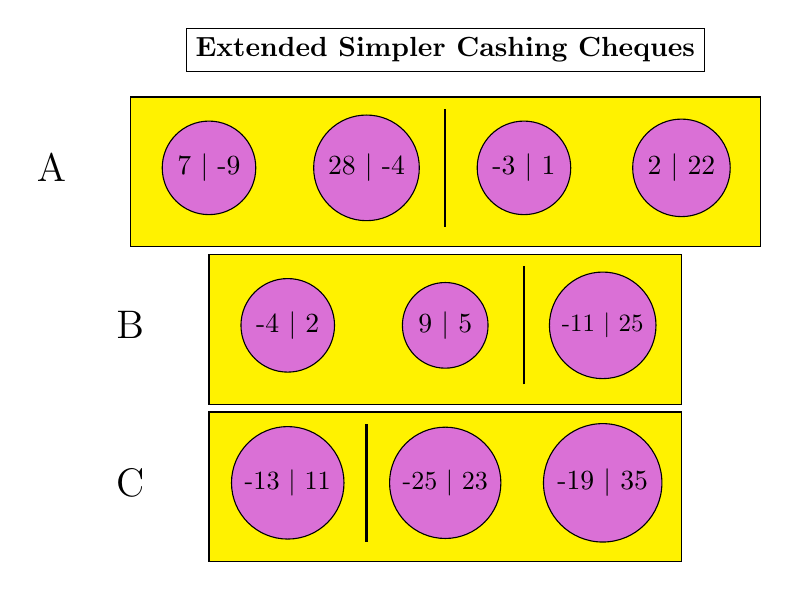
\begin{tikzpicture}
		\node[draw] (title) at (3,1.5) {\textbf{Extended Simpler Cashing Cheques}};
		\begin{scope} []
			\draw[fill=yellow] (-1,-1) rectangle ++(8,1.9);
			\draw[fill=yellow] (0,-3) rectangle ++(6,1.9);
			\draw[fill=yellow] (0,-5) rectangle ++(6,1.9);
			\node[] at (-2,0) {\Large A};
			\node[] at (-1,-2) {\Large B};
			\node[] at (-1,-4) {\Large C};
			\node[circle, draw, fill=purple2] at (0,0) {7 $|$ {-}9};
			\node[circle, draw, fill=purple2] at (2,0) {28 $|$ {-}4};
			\draw[thick] (3,-0.75) -- (3,0.75);
			\node[circle, draw, fill=purple2] at (4,0) {{-}3 $|$ 1};
			\node[circle, draw, fill=purple2] at (6,0) {2 $|$ 22};
			\node[circle, draw, fill=purple2] at (1,-2) {{-}4 $|$ 2};
			\node[circle, draw, fill=purple2] at (3,-2) {9 $|$ 5};
			\draw[thick] (4,-2.75) -- (4,-1.25);
			\node[circle, draw, fill=purple2, scale=0.9] at (5,-2) {{-}11 $|$ {25}};
			\node[circle, draw, fill=purple2, scale=0.95] at (1,-4) {{-13} $|$ 11};
			\draw[thick] (2,-4.75) -- (2,-3.25);
			\node[circle, draw, fill=purple2, scale=0.94] at (3,-4) {{-}25 $|$ 23};
			\node[circle, draw, fill=purple2] at (5,-4) {{-}19 $|$ 35};
		\end{scope}
	\end{tikzpicture}
}
\end{center}
\caption{Sum of hot components without dominated moves}
\end{figure}

It is a good thing now to consider the game above as the sum of three components, $A,B,C$ from top to bottom. It is completely clear what the best moves for left and right are in each of the components. However, from the thermograph of the components, one will find that no moves are dominated, they all influence the resulting thermograph. As seen before, this mean that depending on the ambient temperature the best move in each component will vary.

In the last example, the best move for Left is actually to play in $B$ and make the move to \gam{9}{{-}5}. In this case, the reader should notice that $A + B - 5$ is less negative than the original game, but also that Right will not necessarily move in \gam{9}{{-}5}. Left's move, is an example of taking advantage of the fact the opponent will be distracted moving elsewhere to make the best of, in this case, a bad situation.













    
% Methods
    \chapter{It's all about finding calm in the chaos}
    Although the concepts and definitions of combinatorial game theory have impact in general mathematics, it is a relatively new field of study that has many open problems and not so many resources or implementations available. The purpose of this section is to bring examples, pieces of code and discuss a particular software that implements most of the theory discussed up to this point. The code fragments featured in the text follow C++ syntax, with the intent of being as simple as possible.

The examples and code fragments also serve the purpose of showing possible readers that the theory is actually quite simple, not requiring great mathematical skills, and that applying it is also not difficult. With them, some concepts presented will become clearer and a few facts enunciated will be shown. A second part of this section will introduce a few new games so that the reader might find other interesting games to play. In this second part, the reader will also see that it is not hard to make up fun games on the spot. This section can work as a midpoint between presenting the concepts and a shift in focus to handle the problem of temperature bounding, and may serve to verify if the concepts are clear.

\subsection*{The Numbers}

A very important and recurrent theme in the early parts of the text is the correspondence between games and surreal numbers. It is correct to say that all real numbers are also games, but it may not be clear how to make a particular real number. For example, the reader may not be able to make a game with value equals to $\pi$. In fact, the reader may not know what numbers are easy or hard to do. The first two rules of the simplicity principle should be clear enough.

\begin{lstlisting}[language=C++]
class SurrealNumber {
  public:
	float ToFloat ();
	...
  private:
  	vector<SurrealNumber*> left;
  	vector<SurrealNumber*> right;
  	...
};

float SurrealNumber::ToFloat () {
	float ret;
	if (left.empty())
		if (right.empty())
			ret = 0.0f;
		else
			ret = min(floor(${-}$1 + minRight()->toFloat()), 0.0f);
	else if (right.empty())
		ret = max(floor(1 + maxLeft()->toFloat()), 0.0f);
	// other cases
	...
	return ret;
}
\end{lstlisting}

While easy and hard is relative, every number that is a dyadic rational, a number that is of the form $\frac{a}{2^b}, a\in\mathbb{Z}, b \in \mathbb{N}$ is easy to form. A good method to make the representation of $z = \frac{a}{2^b}, z \ge 0$ in \gam{x}{y} is:\\
\begin{adjustwidth}{2cm}{}
	1) Calculate $d\in \mathbb{Z}\;|\;0 \leq z-d < 1$.\\
	2) If $z=d$ then $x = z-1$ and $y=\emptyset$, stop.\\ 
	3) Binary search for oldest dyadic rational $w$, with $d < w < 1$\\
	4) Save the steps taken in the search \\
	5) $x$ is $d$ added to the oldest number to the left.\\
	6) $y$ is $d$ added to the oldest number to the right.
\end{adjustwidth} \vspace{0.5cm}

For example, $\frac{89}{16} = 5 + \frac{9}{16} = \gam{5 + \frac{1}{2}}{5+\frac{5}{8}}$, because the binary search for \mbox{$\frac{9}{16} = \frac{89-80}{16}$} follows the path $(1\xrightarrow[]{L})\frac{1}{2}\xrightarrow[]{R} \frac{3}{4}\xrightarrow[]{L}\frac{5}{8}\xrightarrow[]{L}\frac{9}{16}$. In RB-Hackenbush, building~$\frac{89}{16}$ is now easy. Take a pile with five blue edges and add it to a blue-red-blue-blue pile. The red-blue-blue pile on top of that derives from the right-left-left path on the binary search for $\frac{9}{16}$, with a right turn corresponding to a red edge and vice-versa.

A similar idea is used in the following featured snippet, but with the objective of finding $z = \frac{a}{2^b}$ given \gam{X}{Y}.

\begin{lstlisting}[language=C++]
	//other cases
	else
		ret = FindSimplesFittingNumber();
	...
}

float SurrealNumber::FindSimplesFittingNumber {
		float maxL = maxLeft();
		float minR = minRight();
		if (maxL < 0 && 0 < minR)
			return 0.0f;
		float d = floor(maxL);
		float x = maxL - d;
		float y = minR - d;
  		float fact = 1.0f;
		while (fact > EPSILON)
			if (x < fact)
				if (y > fact)
					break;
				else
					fact *= 0.5f;
			else
				fact *= 1.5f;
		return d + fact;
	}
\end{lstlisting}

All the remaining numbers are hard in the sense that they require an infinite number of steps to define. A simple code like the one above will not handle that. That is because $\frac{2}{3}$ and $\pi$ are both generated in the $\aleph$th day (section 3), like any other non-dyadic fractions. However, these are not equally hard. Because $\frac{2}{3}$ is a periodic number when using binary representation, its path in the numbers tree is well-defined.

It is true that both $\frac{2}{3}$ and $\pi$ are given by something equivalent to the following: $n = \gam{x \in S_*:x < n}{y \in S_*:y>n}$, where $S_*$ is the set of numbers generated until day $\aleph$. However, $\frac{2}{3}=0.\overline{10}_2$ can also be defined through the infinite right-left-right-left... path in the binary tree, because a 1 in the binary representation is a step do the right in the tree and vice-versa. One way to think of this fact is that, when doing a binary search for $x$ between the dyadics in (0,1), the starting question is $x > 1/2$. The 1 indicates a yes, so the following question is $x > 3/4$, and so on. Since numbers smaller than $x$ go on the left set and vice-versa, $\frac{2}{3} = \gam{1/2, 5/8, \ldots}{3/4,11/16,\ldots}$, showing that the numbers visited in the binary search alternate in the left and right sets. Repeating decimals, in RB-Hackenbush, are extremely easy to spot because they are always a sequence of red and blue edges followed by a finite pattern repeated infinitely.

Other than some real numbers being hard to draw, drawing non-reals is also not trivial. It was shown that there are infinitely many numbers between any two real numbers, in section 3. This might seem hard to understand or accept initially, because the reals form the complete ordered field. However, at least based on Conway surreal numbers, the fact that it is possible to build a game in which the advantage a player has is strictly between two real numbers gives some light to the fact. To do that, simply add an infinitesimal to a real number, as seen before.

\begin{figure}[H]
\begin{center}
	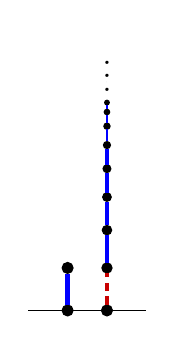
\begin{tikzpicture} 
		\begin{scope} [every node/.style={scale=0.3, style=circle, draw, fill=black}]
			\node [scale=1.4] (1) at (0, -1.80){};
			\node [scale=1.3] (2) at (0, -1.26){};
			\node [scale=1.2] (3) at (0, -0.78){};
			\node [scale=1.1] (4) at (0, -0.36){};
			\node [scale=1]   (5) at (0, 0)      {};
			\node [scale=0.9] (6) at (0, 0.3)  {};
			\node [scale=0.8] (7) at (0, 0.54) {};
			\node [scale=0.7] (8) at (0, 0.72) {};
			\node [scale=0.6] (9) at (0, 0.84) {};
			\node [scale=1.4] (10) at (-0.5, -1.80) {};
			\node [scale=1.4] (11) at (-0.5, -1.26) {};
			\node [scale=0.2, fill=white, draw=none] at (0, 1.1) {$\vdots$};
		\end{scope}
		\draw (-1,-1.80) -- (0.5, -1.80);
		\draw[red, densely dashed, ultra thick] (1)--(2);
		\draw[blue, ultra thick] (2)--(3);
		\draw[blue, ultra thick] (3)--(4);
		\draw[blue, ultra thick] (4)--(5);
		\draw[blue, ultra thick] (5)--(6);
		\draw[blue, thick] (6)--(7);
		\draw[blue, thick] (7)--(8);
		\draw[blue] (8)--(9);
		\draw[blue, ultra thick] (10)--(11);
		\node[scale=1.5] at (0, 1.3) {\scriptsize$\vdots$};
	\end{tikzpicture},
\end{center}
\caption{Drawing non-reals is not hard}
\end{figure}

The game in the figure has value $1-\epsilon$, a number smaller than 1, but larger than any $x \in \mathbb{R}, x < 1$. Although the non-reals might be new, the effort of writing hard reals and non-reals as RB-Hackenbush is very similar.

RB-Hackenbush is an extremely good example to understand numbers, as finding dyadics and repeating decimals are very easy. However, not all games are like this. It was shown that
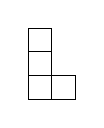
\begin{tikzpicture}
	\draw[] (0.3,-0.3) rectangle ++(0.3,0.3);
	\draw[] (0,-0.3) rectangle ++(0.3,0.3);
	\draw[] (0,0) rectangle ++(0.3,0.3);
	\draw[] (0,0.3) rectangle ++(0.3,0.3);
\end{tikzpicture} = $\frac{1}{2}$, but how would one build an instance of $\frac{1}{4}$, or $\frac{1}{2^n}$, for $n\in\mathbb{N}$? It turns out that it is not trivial at all.

In fact, only in 1996 a partial solution was given. One of the results of the paper ``New Values in Domineering" \cite{10} was the existence of arbitrarily small values of domineering games. Before that, it was unknown whether or not they existed. It was only in 2015 \cite{11} that a method to create all dyadic rationals in a single component was introduced. Following the strategy presented in 1996, the so-called Yonghoan Kim's snakes were created, named after the author. The snake's representation is found below, copied from Richard K. Guy's list of unresolved problems in \textit{Games of no Chance} \cite{GONC}:

\vspace{1cm}\hspace{-2cm}
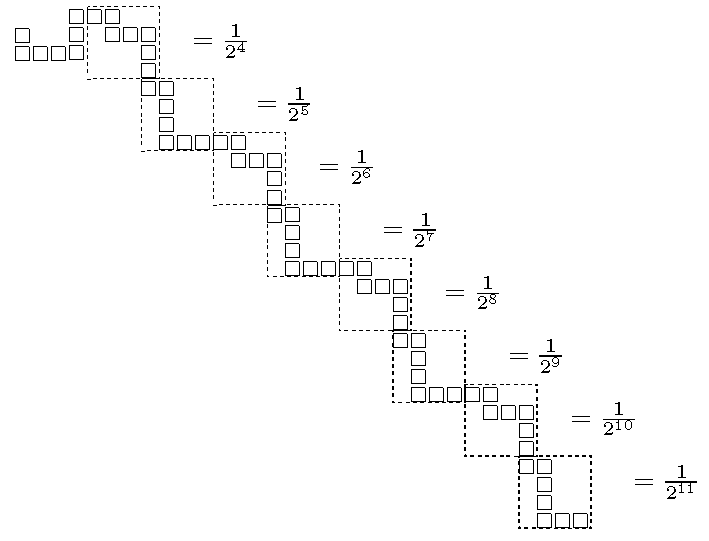
\includegraphics[scale=0.9]{../images/kims_snakes.png}

In this method of finding dyadics, there is a initial structure, that is not marked by a dashed rectangle. To this structure, additional ones are appended. As shown, each additional structure alternated between two others. Of course that the resulting game is not the only game with the given values.

In fact, there are special games with the same value as the snakes. The 2015 paper is based on these special games. The special games are based on concatenating and imploding bridges in domineering games. Bridges are cells that do not change the value of a game, and are also called explosives squares. For example, 
\begin{tikzpicture}
	\draw[] (0.3,0) rectangle ++(0.3,0.3);
	\draw[] (0,0) rectangle ++(0.3,0.3);

\end{tikzpicture}
and
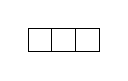
\begin{tikzpicture}
	\draw[] (0.9,0) rectangle ++(0.3,0.3);
	\draw[] (1.2,0) rectangle ++(0.3,0.3);
	\draw[] (1.5,0) rectangle ++(0.3,0.3);
\end{tikzpicture}
have the same value, so one of the extremities is a bridge. The strategy is built upon two theorems that are beautiful because they are powerful yet very simple.

The \textit{Bridge Splitting Theorem for Domineering} was introduced by Conway's. It reads:
If the value of \Gm{}\begin{tikzpicture}\draw[] (0.1,0) rectangle ++(0.3,0.3);\end{tikzpicture} is the same as \Gm{}, then the value of \Gm{}\begin{tikzpicture}\draw[] (0.1,0) rectangle ++(0.3,0.3);\end{tikzpicture}\Hm{} is the sum of the values of \Gm{} and \begin{tikzpicture}\draw[] (0.1,0) rectangle ++(0.3,0.3);\end{tikzpicture}\Hm{}, given \Gm{} and \Hm{} do not intersect. The proof is:

$$
\Gm{}\begin{tikzpicture}\draw[] (0.1,0) rectangle ++(0.3,0.3);\end{tikzpicture}\Hm{} \leq \Gm{} + \begin{tikzpicture}\draw[] (0.1,0) rectangle ++(0.3,0.3);\end{tikzpicture}\Hm{} = 
\Gm{}\begin{tikzpicture}\draw[] (0.1,0) rectangle ++(0.3,0.3);\end{tikzpicture} + \begin{tikzpicture}\draw[] (0.1,0) rectangle ++(0.3,0.3);\end{tikzpicture}\Hm{} \leq
\Gm{}\begin{tikzpicture}\draw[] (0.1,0) rectangle ++(0.3,0.3);\end{tikzpicture}\Hm{}
$$

The first inequality since splitting a horizontal always favors Right, and, the second inequality is true because merging horizontal squares also always favors Left. The second important theorem was created by the authors.

\textit{Bridge Destroying Theorem for Domineering}

If the value of \Gm{}\begin{tikzpicture}\draw[] (0,0) rectangle ++(0.3,0.3);\end{tikzpicture}, 
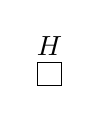
\begin{tikzpicture}\draw[] (0,0) rectangle ++(0.3,0.3);\node at (0.15, 0.5) {$H$};\end{tikzpicture}, 
\begin{tikzpicture}\draw[] (0.1,0) rectangle ++(0.3,0.3);\end{tikzpicture}$I$
 and
\begin{tikzpicture}[baseline={(current bounding box.center)}]\draw[] (0,0) rectangle ++(0.3,0.3);\node at (0.15,-0.2){$J$};\end{tikzpicture}
 are the same of the values of $G$, $H$, $I$, $J$, then the value of
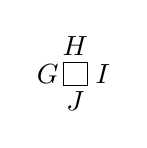
\begin{tikzpicture}[baseline={(current bounding box.center)}]
	\draw[] (0,0) rectangle ++(0.3,0.3);
	\node at (-0.2, 0.15) {$G$};
	\node at (0.15, 0.5) {$H$};
	\node at (0.5, 0.15) {$I$};
	\node at (0.15,-0.2){$J$};
\end{tikzpicture}
is the same as the sum of $G, H, I$ and $J$, provided that neither of the games have common edges. The proof is also simple:

$$
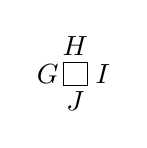
\begin{tikzpicture}[baseline={(current bounding box.center)}]
	\draw[] (0,0) rectangle ++(0.3,0.3);
	\node at (-0.2, 0.15) {$G$};
	\node at (0.15, 0.5) {$H$};
	\node at (0.5, 0.15) {$I$};
	\node at (0.15,-0.2){$J$};
\end{tikzpicture} \leq
G + 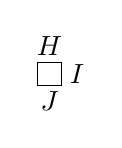
\begin{tikzpicture}[baseline={(current bounding box.center)}]
	\draw[] (0,0) rectangle ++(0.3,0.3);
	\node at (0.15, 0.5) {$H$};
	\node at (0.5, 0.15) {$I$};
	\node at (0.15,-0.2){$J$};
\end{tikzpicture} \leq
G + I + 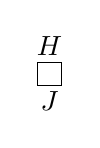
\begin{tikzpicture}[baseline={(current bounding box.center)}]
	\draw[] (0,0) rectangle ++(0.3,0.3);
	\node at (0.15, 0.5) {$H$};
	\node at (0.15,-0.2){$J$};
\end{tikzpicture} =
G + H + I + J =
$$
$$
= H + J + 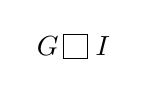
\begin{tikzpicture}[baseline={(current bounding box.center)}]
	\draw[] (0,0) rectangle ++(0.3,0.3);
	\node at (-0.2, 0.15) {$G$};
	\node at (0.5, 0.15) {$I$};
\end{tikzpicture} \leq
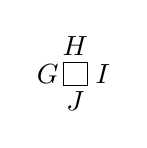
\begin{tikzpicture}[baseline={(current bounding box.center)}]
	\draw[] (0,0) rectangle ++(0.3,0.3);
	\node at (-0.2, 0.15) {$G$};
	\node at (0.15, 0.5) {$H$};
	\node at (0.5, 0.15) {$I$};
	\node at (0.15,-0.2){$J$};
\end{tikzpicture}
$$

The first two inequalities are true because they both split a horizontal line, favoring right. The two equalities are true because they are applications of the \textit{Bridge Splitting Theorem for Domineering}. The last inequality is true because it is a linking of a vertical line, which can only favor Left.

An example of applying this is figuring out that 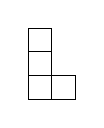
\begin{tikzpicture}
	\draw[] (0.3,-0.3) rectangle ++(0.3,0.3);
	\draw[] (0,-0.3) rectangle ++(0.3,0.3);
	\draw[] (0,0) rectangle ++(0.3,0.3);
	\draw[] (0,0.3) rectangle ++(0.3,0.3);
\end{tikzpicture} =
\begin{tikzpicture}
	\draw[] (0.3,-0.3) rectangle ++(0.3,0.3);
	\draw[] (0,-0.3) rectangle ++(0.3,0.3);
	\draw[] (-0.3,-0.3) rectangle ++(0.3,0.3);
	\draw[] (0,0) rectangle ++(0.3,0.3);
	\draw[] (0,0.3) rectangle ++(0.3,0.3);
\end{tikzpicture} = $\frac{1}{2}$, therefore it is true that 
\begin{tikzpicture}
	\draw[] (0.3,-0.3) rectangle ++(0.3,0.3);
	\draw[] (0,-0.3) rectangle ++(0.3,0.3);
	\draw[] (-0.3,-0.3) rectangle ++(0.3,0.3);
	\draw[] (0.6,-0.3) rectangle ++(0.3,0.3);
	\draw[] (0.9,-0.3) rectangle ++(0.3,0.3);
	\draw[] (0,0) rectangle ++(0.3,0.3);
	\draw[] (0,0.3) rectangle ++(0.3,0.3);
	\draw[] (0.6,0) rectangle ++(0.3,0.3);
	\draw[] (0.6,0.3) rectangle ++(0.3,0.3);
\end{tikzpicture} $=1$. Another, much more beautiful example is given on 2015 paper:

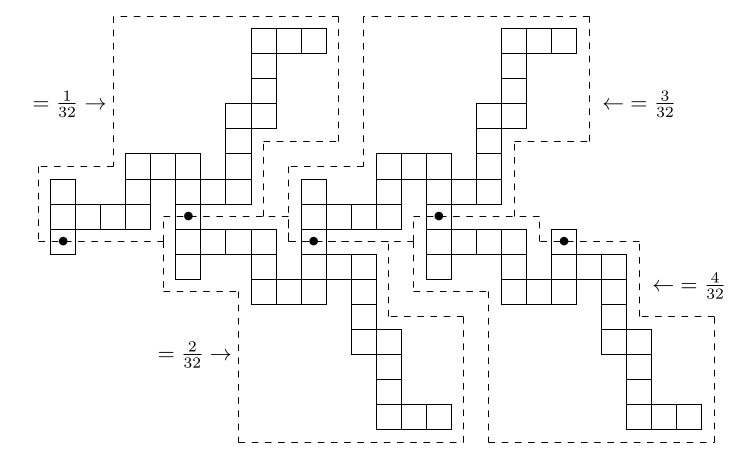
\includegraphics[scale=0.5]{../images/dyadic_domineering.png}

By combining the two theorems with Kim's snakes, it would be possible to create any dyadic in a single connected component, if not for two problems. The first is the problem of creating a bridge. However, that is a non-problem because Kim's snakes always have explosive squares. An explosive square that is always there is a square below the two vertical squares to the left of the base configuration of Kim's snakes. Since the value of the snake is equal to the values of the sum of the bridged components, the base component may be interchanged with the one with an explosive square and the values of the snake would remain the same.

The second problems is that of making sure ever component will not share an edge with the others. The solution of this second problem is fond on the aforementioned paper. The domineering discussion above serves to show how some games are good to analyse and create examples with, while other not so much. RB-Hackenbush is great for working with numbers and ``Extended Simpler Cashing Cheques" (ESCC) is provides a great ruleset to work with temperature. 

\subsection*{The non-numbers}

When the topic changed from numbers to non-numbers, an example of ambient temperature, and how it affected play, was required. In order to keep the results to the boundaries of the literature, an instance of this game was showed. This instance was made by reverse engineering the example of the same topic found on \textit{Winning Ways} \cite{WW} in this convenient game. Normally, it is extremely hard to generate a configuration with any temperature value, but ESCC allows it, and this is why its creation in this text was important.

ESCC allows an easy conversion from a \gam{X}{Y} to a configuration, mainly because any switch is trivial to write down. The thermograph found in the \textit{Winning Ways} book is copied below:

\vspace{0.5cm}\hspace{-1.5cm}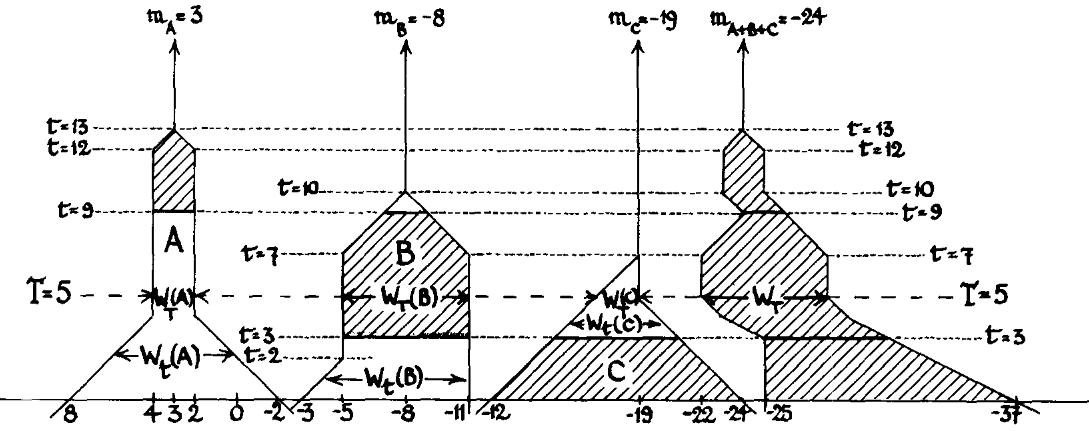
\includegraphics[scale=0.45]{../images/cpd_therm_ww.png}
\vspace{0.5cm}

To verify that the resulting compounded thermograph of the example featured in the previous section is indeed the one found above, it is possible to use Aaron Siegel's CGSuite. CGSuite is an implementation of almost all of the methods found in Combinatorial Game Theory. This text will not go in detail on the software package, but Appendix A brings to light some additional information.

Between other practical and interesting features, it is possible to create any games and calculate and plot their thermographs. For example:

\begin{center}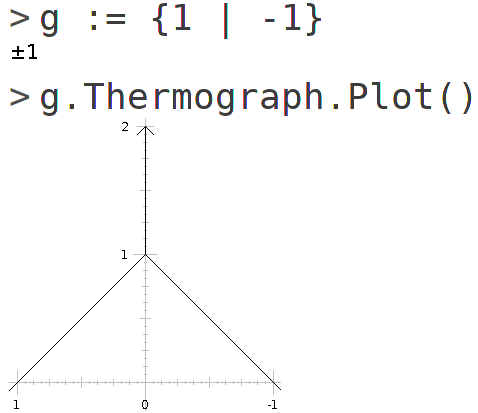
\includegraphics[scale=0.3]{../images/cgsex1.png}\end{center}

The game from last section could, then, be converted to the following:

\begingroup
\tikzset{every picture/.style={scale=0.5}, every node/.style={scale=0.5}}%
\begin{figure}[H]
\begin{center}
	\scalebox{0.9}{
	\begin{tikzpicture}
		\node[draw] (title) at (3,1.5) {\textbf{Extended Simpler Cashing Cheques}};
		\begin{scope} []
			\draw[fill=yellow] (-1,-1) rectangle ++(8,1.9);
			\draw[fill=yellow] (0,-3) rectangle ++(6,1.9);
			\draw[fill=yellow] (0,-5) rectangle ++(6,1.9);
			\node[] at (-2,0) {\Large A};
			\node[] at (-1,-2) {\Large B};
			\node[] at (-1,-4) {\Large C};
			\node[circle, draw, fill=purple2] at (0,0) {7 $|$ {-}9};
			\node[circle, draw, fill=purple2] at (2,0) {28 $|$ {-}4};
			\draw[thick] (3,-0.75) -- (3,0.75);
			\node[circle, draw, fill=purple2] at (4,0) {{-}3 $|$ 1};
			\node[circle, draw, fill=purple2] at (6,0) {2 $|$ 22};
			\node[circle, draw, fill=purple2] at (1,-2) {{-}4 $|$ 2};
			\node[circle, draw, fill=purple2] at (3,-2) {9 $|$ 5};
			\draw[thick] (4,-2.75) -- (4,-1.25);
			\node[circle, draw, fill=purple2, scale=0.9] at (5,-2) {{-}11 $|$ {25}};
			\node[circle, draw, fill=purple2, scale=0.95] at (1,-4) {{-13} $|$ 11};
			\draw[thick] (2,-4.75) -- (2,-3.25);
			\node[circle, draw, fill=purple2, scale=0.94] at (3,-4) {{-}25 $|$ 23};
			\node[circle, draw, fill=purple2] at (5,-4) {{-}19 $|$ 35};
		\end{scope}
	\end{tikzpicture}
}
\end{center}
\caption{Sum of hot components without dominated moves}
\end{figure}
\endgroup
\begin{center}
	$\Downarrow$
\end{center}
\begin{figure}
\begin{center}
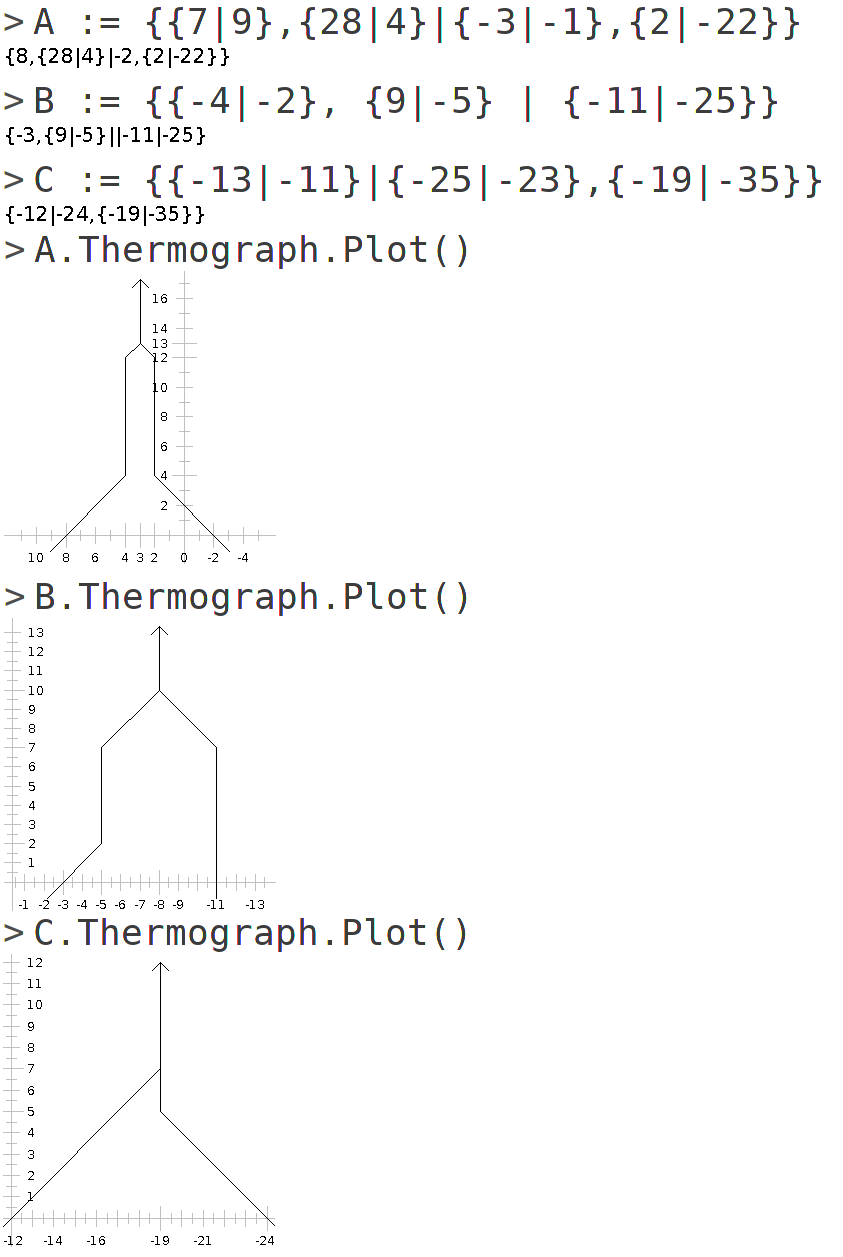
\includegraphics[scale=0.3]{../images/resulting_thermographs.png}
\end{center}
\caption{Thermographs of the components named A, B and C}
\end{figure}

Therefore the game from last section is indeed the same as the one featured in the book. The steps taken to reverse engineer the games whose thermographs were the ones indicated in the book, might be useful to speed up the process of calculating and exercising the process of building thermographs by head. This process uses a theorem not yet mentioned.

This theorem is about the structure of thermographs. It states that every line in a thermograph has slope equals to ${-}1$, $0$ or $1$ and masts have slope 0. Using the notation created by Aaron \cite{CGT}, let $G$ be a game and $\lambda_t(G), \rho_t(G)$ its thermograph's left and right trajectories, respectively. It means that:

\begin{align*}
\overset{\sim}{\lambda}_t(G) =&\; \underset{G^L}{max}(\rho_t(G^L)- t)\\
\overset{\sim}{\rho}_t(G) =&\; \underset{G^R}{min}(\lambda_t(G^R) + t)\\
\lambda_t(G) = \overset{\sim}{\lambda}_t(G),\;\rho_t(G) =& \overset{\sim}{\rho}_t(G)\text{ if $t$ bellow the freezing point.}
\end{align*}

As seem before, for any temperature above the freezing point, the values of the left and right slants are the same and do not change. 

(a) Every segment of $\lambda_t(G)$ has slope 0 or ${-}1$.

(b) Every segment of $\rho_t(G)$ has slope 0 or $1$.

(c) Both trajectories have masts of slope 0, with the same value.

The proof is not complicated. First the proof of (a) and (b), given via induction:

\textit{Base:} (a) and (b) are true if $G$ is a number, as the slope is always zero.

\textit{Induction Step:} Let $\lambda_t(G^R)$ satisfying (a) and $\rho_t(G^L)$ satisfying (b). Since, by definition, \mbox{$\overset{\sim}{\lambda}_t(G) =\; \underset{G^L}{max}(\rho_t(G^L)- t)$}, the slope of $\overset{\sim}{\lambda}_t(G)$ is either 0 or 1 translated by ${-}t$. The same goes for $\overset{\sim}{\rho}_t(G)$. Since \mbox{$\overset{\sim}{\rho}_t(G) =\; \underset{G^R}{min}(\lambda_t(G^R) + t)$}, the slope of $\overset{\sim}{\lambda}_t(G)$ is either ${-}1$ or 0 translated by ${+}t$. This way, (a) and (b) are true.

Now, the proof of (c), also via induction. Notice that this part proves the existence of a freezing point, and the mast follows by definition.

\textit{Base:} (c) is true if $G$ is a number, as the slope is always zero.

\textit{Induction Step:} Let the slopes of $\lambda_t(G^R)$ and $\rho_t(G^L)$ be zero. Therefore, the masts of $\overset{\sim}{\lambda}_t(G)$ and $\overset{\sim}{\rho}_t(G)$ are ${-}1$ and ${+}1$ respectively. Since $\overset{\sim}{\lambda}_t(G) \leq \overset{\sim}{\rho}_t(G)$, the left and right trajectory cross and, therefore, there is a freezing point. By definition, after the freezing point, the slope is zero.

If the reader goes through the thermographs in this text, he/she will notice that this is indeed true for the examples. Trying to find a counter-example may help understand the proof, as inevitably, the recursive definition of the thermograph always leads to the base case of number's thermographs. Now that this rules are properly stated, it is possible to understand how to write a game \Gm{=\gam{X}{Y}} based on an existing thermograph.

Starting by the thermograph of $C$, it is easy to spot that there is only one viable option for Left. Since the left slant, $\overset{\sim}{\lambda}_t(G)$, of that graphic has slope ${-1}$, then $\rho_T(G)$ has slope 0. Since the slant crosses the x-axis in $x={-12}$, then an option to this Left option is the number ${-12}$. The option then, is the canonical form of this number, adapted to fit the rules of the cashing cheques game. The right trajectory is a bit more complicated.

Starting with the inclined slant, the procedure described above helps one finding out that the number ${-24}$ is enough. The vertical line between the bent line and the freezing point must come from a non-number. Because a bent line added to the cooling factor $t$ is a straight line, then the left slant of this non-number must cross the x-axis in $x={-19}$. Another requirement is that this game must be hot until $t=7$, because the straight line goes until this point. With this in place, it is possible to create the game \gam{{-19}}{{-35}}, because ${-35} = {-19} - 7 - 7$, in which the sevens come from the $t=7$ and are used twice because the cooling happens in both directions. In this example, the right option could be any number smaller than ${-35}$, because the boiling point would remain the same

The thermograph of $B$ is more difficult. The first bent line of the left trajectory is the same as before, and, in this case, the number ${-3}$ is enough. The straight line, just like before, comes from a non-number whose right option is ${-5}$. Unlike the non-number from the previous example, however, the freezing point of this case must be exactly 7, so the distance between the right and left stops must be 14, unlike the previous example. With this information, it becomes possible to build the game \gam{9}{{-5}}. The last bent segment is the mast of the non-number.

The right trajectory of $B$ is the simplest \gam{{-11}}{{-25}}, which has already been explained. The process to build the game $A$ is a repetition of the left left trajectory of $B$ for both the left and right trajectories. By going through this, hopefully it became clear that thermographs are not hard to build. Also, by using the same example as the book, the reader might also benefit from the remarks found there.

Just like RB-Hackenbush is a very good game to build example of numbers, Extended Simpler Cashing Cheques is a very good game to build examples of temperature. The brief description of how to build dyadics in domineering and how long it took for the process to be created, showed that domineering is not a good game to study numbers. Up to this point domineering has been used to exemplify the study of temperature, but the truth is temperature in domineering is limited, both in numerical values and in current knowledge of the game.

In fact, in 2005 two researches brought to light that Elwyn Berlekamp conjectured, in 2004, that the maximum temperature in domineering is 2. That is yet to be proven or disproved, although computed instances also lead to the same conclusion. It may not be all that clear yet, but many common games cannot have arbitrarily high temperatures. In a domineering position with temperature two, whoever plays first finishes with two spare moves. Before trying to create such a position, the intricacies of such a position might not be clear.

In 2004 an instance of that position was found, and that was the only one, in a connected board of course, up to this day. While this conjecture is a typical open problem in combinatorial game theory, there are not many attempts to solve this. The next section is dedicated a PhD thesis that gave an upper bound for certain configurations in domineering, although that does not answer the question.

\subsection*{It is simple but not easy}

The initial code fragment of the section only dealt with simple surreal numbers, even making a lot of assumptions about left and right, without verifying anything. It might make sense to think about how one would implement, in practice, the numerical part of a library like CGSuite. Considering only the SurrealNumber class, if the only available method of defining numbers were the left and right sets, how would be the simple number $3 = \gam{2}{}$ be written?

Of course that, with only that available, the recursive structure of surreal numbers \gam{\gam{\gam{\gam{}{}}{}}{}}{}. Although correct according to the theory, implementing number like that, only, would cause problems because evaluating a number would no be a trivial operation. For instance, telling whether $2.5 = \gam{2}{3} < 3 = \gam{2}{}$ would require traversing both number's left and right trees. The canonical representation of the number 3, for example, would be something like this:

\begin{figure} [H]
\begin{center}
\begin{tikzpicture}
	[
	level distance=30pt,
	level 1/.style={sibling distance=4cm},
	level 2/.style={sibling distance=1.7cm},
	every node/.style = {
	},
	every child/.style = {
		ultra thick
	}
	]
{
\node{num (3)}
	child{node{left}
		child[->]{node{num(2)}
			child[-]{node{left}
				child[->]{node{num(1)}
					child[-]{node{left}
						child[->]{node{num(0)}
							child[-]{node{left}}
							child[-]{node{right}}}}
						child[-]{node{right}}}}
				child[-]{node{right}}
	}}
	child{node{right}};
}
\end{tikzpicture}
\end{center}
\end{figure}

Given this problems, a viable implementation of combinatorial games must look for alternative representations. Some possibilities are allowing surreal numbers to be represented with integers and floats or to store results of the tree traversals to minimize the number of times the complex tree structure must be analyzed. When looking at numbers strictly, the tree that resulted in a float or another chosen numerical representation may be discarded because it does not contain special information.

However, when changing the domain from surreal numbers to games, the tree cannot be always discarded. The reason for that is that the game tree may contain relevant information for gameplay. One could try keeping only the best move for each position in order to save space. However, as seen before, adding games may change which move is best so not all branches can be discarded.

Consider the following draft of a combinatorial game class declaration:

\begin{lstlisting}
// CombinarotialGame.hpp
#include "everything_required.hpp"
using namespace std;

class CombinatorialGame {
  public:
	CombinatorialGame (vector<CombinatorialGame*> l,
					     vector<CombinatorialGame*> r);
	...
  private:
  	vector<CombinatorialGame*> left;
  	vector<CombinatorialGame*> right;
  	bool isSurreal;
  	bool isSwitch;
  	float realValue;
  	float bias;
  	float temperature;
};

\end{lstlisting}

\begin{lstlisting}
//CombinatorialGame.cpp
#include "path/to/CombinatorialGame.hpp"

CombinatorialGame::CombinatorialGame (
                    vector<CombinatorialGame*> l,
                    vector<CombinatorialGame*> r) {
	float maxL, minR;
	bool lFlag, rFlag;           
}
	
\end{lstlisting}

Implementing the draft above woulds help with space requirements and unnecessary calculations but does not completely solve any of the more complex issues. It would, for example, avoid repeated calculations, unlike the version where the GetFloat method went through the game tree calculating it on demand.

However, for one, an implementation of this draft would be incapable of handling infinite games, as those cannot be stored in vectors. Again, a more complete version can be found in CGSuite github repository, but understanding and tackling the difficulties may be a worth exercise. Even that package used by many researches has it issues and does not deal well with infinity either.

\subsection*{Other Games To Play}

Now that vocabulary, methods and tools were introduced, this section brings some games to put your knowledge to proof.

\textbf{The Amazons} is a typical game that, like domineering, is fun and only requires pen and paper. Amazons is typically played in a 10x10 chess board with each player having four initial pieces in the fixed initial position depicted below. Each piece works just like a chess queen. In each turn, the player selects one of his/her queens and moves in an arbitrarily number of squares, like the regular chess queen. After moving, the amazon has to shoot an arrow in any direction however many cells desired. The arrow burns the cell. The amazon and the arrow cannot go through any burned square, and this is what makes the game interesting.

A common variation is one where every square the amazon (queen) goes through is then burned from the game, making it so that no queen can move over it. Burning the path either amazon goes through is a replacement for shooting the arrows and there are many other possibilities, like shooting two arrows or shooting and burning the path, or choosing either of those.

In either variation, like in most short games, the initial position in unimportant and the players can choose any starting position they find interesting.

\begin{figure} [H]
	\begin{center}
		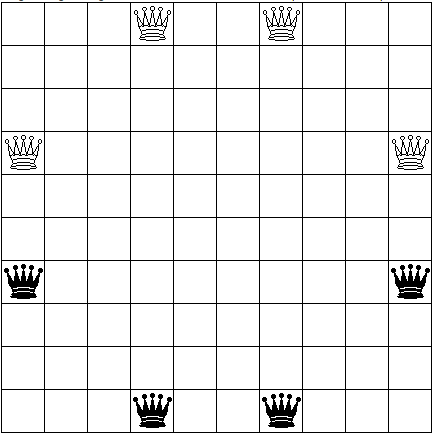
\includegraphics[scale=0.5]{sections/examples/amazons.png}
	\end{center}
\caption{Most typical starting positions in Amazons}
\end{figure}

For example, play may take place in an 8x8, a chessboard for convenience, with each player having two queen in opposing corners. Since, in this example, player Left is a beginner an Right is a seasoned player, Left has one additional queen next to one of his/her queens. It serves to show that there are no restrictions to the initial position - games do not have to be mathematically balanced to be fun.

\begin{figure} [H]
	\begin{center}
		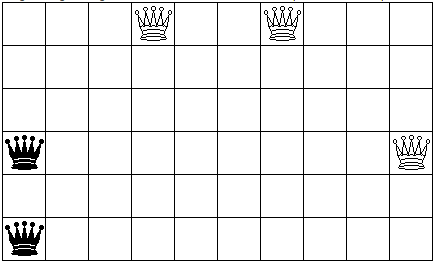
\includegraphics[scale=0.5]{sections/examples/unbalanced_amazons.png}
	\end{center}
	\caption{Unbalanced and fun position in Amazons}
\end{figure}

\textbf{The Angel Game} is more of a mathematical challenge more than a game, because it is not meant to actually be played. This game is played in a infinite squared board, with the Angel being located in of its cells. Each turn the Angel flies over $k$ squares and lands, depending on the desired rules. When it is the devils turn to play, it possesses a square from the infinite board. The challenge is to know whether, and for what values of $k$, the devil wins, given the Angel may not lend in a possessed square. It is clear that this game, depending on the parameters and variations, may not be a short game.

This game led to a lot of research until it was solved. Although it may not interest someone looking for a fun game it serves to show that even games on infinite boards are part of this theory. An important aspect of this game is that the position, after every move, becomes better and better for the devil, but still, sometimes it does not improve enough for the devil to win, even after an arbitrarily large number of moves.

\textbf{Snorts} is yet another fun game to be played with pen and paper. Snorts is a picture coloring game. Two herdsman, Bob, that has a herd of bulls, and Chad, that has a herd of cows, compete to buy properties in a large open field. They are both interested in acquiring as many properties as possible, regardless of their sizes, but they respect each others space. Since cows cannot live next to bulls and vice-versa, Bob and Chad cannot buy any property next to each other.

The initial position for playing snorts any collection of shapes. The initial position is somewhat problematic to draw, because may cause the first player to have easier time playing. However, by making a large initial open space, it is harder to make a boring game. A good method to draw the board is to make a circle-like shape and start partitioning it randomly, making sure that there are not very large partitions. The picture below is an example of a snorts game in progress.

\begin{figure} [H]
	\begin{center}
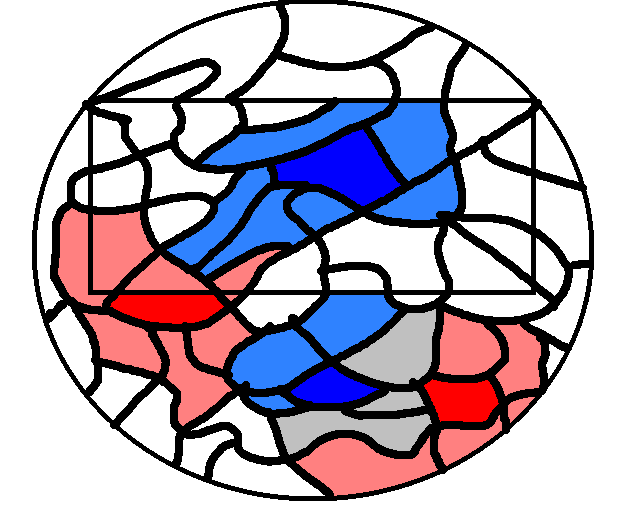
\includegraphics[scale=0.6]{sections/examples/snorts.png}
	\end{center}
\caption{Ongoing match of snorts}
\end{figure}

\textbf{The Knights} is another possible variation of Amazons. The game has the same rules but uses chess knights instead of chess queens. This game may, for experienced chess players, seem less fun that the amazons, as it is much more predictable. It may be true, but, like the other variations of amazons it may be worth trying.















    
% Empirical Analysis
    \chapter{An amazing result and a dive into algebra}
    As the name suggests, this section has a different focus compared to the previous. This sections is concerned of classifying a few games, both in terms of gameplay and in terms of algebraic structure. This important because highlights important characteristics in underlying structure and in possible values.

This sections features a few theorems that end up proving an upper bound for the boiling point of classes of games.

\subsection*{The Result}

The temperature's upper bound results from a through analysis of the thermograph. \todo{quote} brings the first of such results, although the content featured first in Svenja's PhD thesis in 2018. The proof of the boiling point requires a few smaller results and all the required content is summarized in the remaining of this subsection.

The confusion interval of a game is the range of numbers with which it is confused. A game is confused with a number if it is neither greater, smaller nor equal to that number. Any game with temperature greater than 0 is confused with numbers. Take any instance of such cases from previous sections to verify that their confusion interval includes all numbers between the points where the thermograph intersects the $t=0$ line. Some intervals also include either one or both of the intersection points, depending on what the thermograph look below that line.

However, the reader can also verify that some non-numbers with temperature 0 are also confused with numbers. Section four shows that the thermograph of \gam{0}{0} is different to that of 0, although above the $y=0$ they are the same. However, if using the surreal $<$ operation defined in chapter 3, one notices that $\gam{0}{0} \not\lessgtr 0$. However, not all non-numbers behave this way, because some fall in gaps, as seem in section 3. \gam{0}{\gam{0}{0}} is such a game and it is said that its confusion interval does not contain any numbers.

The confusion interval of \Gm{} is usually indicated by $\ell(G)$ and the intersection points are usually denoted by $LS(G)$ and $RS(G)$, and called left and right stops. Therefore $\ell(G) = LS(G)-RS(G)$. Another important definition is the thermic version of a game. The thermic version of a game \Gm{} is a game $\tilde{\Gm{}}$ with the same temperature of \Gm{} but with only one left and one right option, that are also left and right options for \Gm{}. \todo{maybe rephrase}.

\textit{Theorem:} If \Gm{} is hot, then there exists a \Gm{^L} and a \Gm{^R} such that $t(G) = t(\gam{\Gm{^L}}{\Gm{^R}})$. The proof is simple: the mast of \Gm{} begins where the cooled thermographs of some of the left and right options first intersect. There are possibly many left and right options that intersect on the same point. By taking any one of them, \Gm{^{L_+}} and \Gm{^{R_+}}, it is clear that the thermic version of a game exists, because $t(G) = t(\gam{\Gm{^{L_+}}}{\Gm{^{R_+}}})$.

Finding in practice the thermic version of game is not at all simple. In fact, without additional information of \Gm{}, it would be needed to build the entire thermograph, or equivalent information, beforehand. This is an important consideration, that is also made on Dr. Huntemann thesis, but one that is not problematic. Soon, the bound will be created for \Gm{} directly, so that finding the thermic version is not necessary.

It is trivial but it is worth highlighting that the thermograph of \Gm{} and that of $\tilde{\Gm{}}$ may not be the same. In particular $\lambda_t(\tilde{\Gm{}}) \ge \lambda_t(\Gm{})$ and $\rho_t(\tilde{\Gm{}}) \leq \rho_t(\Gm{})$. If it is not clear why the observation is true: for any temperature $t$, the trajectories of the thermograph were either the maximum/minimum of all the corresponding options. The selected left and right options for the thermic version of \Gm{} are only the minimum/maximum for temperatures close to the boiling. Therefore the initial trajectory might be different, but is always lesser/greater or equal to the thermic trajectories.

Using the notation described above it may be simpler. $\lambda_t(\Gm{}) = LS(\Gm{_t}) = max_{\Gm{^L}}(RS(\Gm{^L_t}) - t)$. Since $\Gm{^{L_+}} \in \Gm{^L}$, it is clear that $\lambda_t(\tilde{\Gm{}}) \ge \lambda_t(\Gm{})$. An equivalent statement can be made for the right trajectory.

A result, when fixating $t=0$ is:

\begin{align*}
\ell(\tilde{\Gm{}}) \leq& \ell(\Gm{})\\
\text{Since } \ell(\tilde{\Gm{}}) = LS(\tilde{\Gm{}}) - RS(\tilde{\Gm{}})\leq& LS(\Gm{}) - RS(\Gm{}) = \ell(\Gm{})
\end{align*}

The thermograph, as described in the previous section, is composed of straight lines and $\pm$45$\deg$ oblique lines. The bound is based on this and the size of the confusion interval. Before proceeding, one additional definition.

Let $T^L$ be the sequence $(0, t_1, t_2, \ldots, t_k)$ of the temperatures of the turning points of $\lambda(\tilde{\Gm{}})$. Let, now, $A^L$ be the sequence $(a_0, a_1, \ldots, a_k)$ of labels given by:

\hspace{2cm}$
\begin{cases}
a_i $ is \textit{vertical} if $ \rho(\tilde{\Gm{}}^L_{t_{i+1}}) = \rho(\tilde{\Gm{}}^L_{t_i})\\
a_i $ is \textit{oblique} if $ \rho(\tilde{\Gm{}}^L_{t_{i+1}}) < \rho(\tilde{\Gm{}}^L_{t_i})
\end{cases}
$

Lastly,

\hspace{2cm} $T^L_{\text{V}} = \sum\limits_{\substack{i\;|\;a_i \text{ is} \\ \text{vertical}}}(t_{i+1} - t_i)$

\hspace{2cm} $T^L_{\text{O}} = \sum\limits_{\substack{i\;|\;a_i \text{ is} \\ \text{oblique}}}(t_{i+1} - t_i)$

Notice that the right counterpart can be done similarly. Essentially, $T^L_{\text{V}}$ is the length of the vertical segments and $T^L_{\text{O}}$ is the length of the oblique segments. Of course

\begin{align*}
	t(\Gm{}) =& T^L_{\text{V}} + T^L_{\text{O}}.\\
	&\text{and} \\
	\ell(\tilde{\Gm{}}) =& T^L_{\text{O}} + T^R_{\text{O}}.
\end{align*}

\textit{The theorem} is the following:

Given \Gm{} and $\tilde{\Gm{}}$ its thermic version, then

$$
t(\Gm{}) \leq \ell(\Hm) + \frac{\ell(\Gm{})}{2}
$$

where $\Hm = \tilde{\Gm{}}^L$ if $T^L_V \ge T^R_V$, otherwise $\Hm = \tilde{\Gm{}}^R$. For simplicity, the proof considers that $\Hm = \tilde{\Gm{}}^L$, but again, an equivalent procedure proves the other case.

The length of $T^L_V$ is at most the length of the oblique segments of $\rho(\tilde{\Gm{}}^L)$. Notice that it could be smaller because the left and right options might intersect before the mast of $\tilde{\Gm{}}^L$. In any case, it is clear that the length of this oblique segments is at most the same size of the confusion interval of$\tilde{\Gm{}}^L$. It could be smaller in case there are oblique segments in $\lambda(\tilde{\Gm{}}^L)$.

Therefore, $T^L_V \leq \ell(\tilde{\Gm{}}^L)$

Additionally:

\begin{align*}
T^L_V + T^L_O =&\;T^R_V+T^R_O\\
\text{Since, in this case, }& T^L_V \ge T^R_V\text{:}\\
T^L_O \leq&T^R_O
\end{align*}

Therefore:

\begin{align*}
	2\times T^L_O \leq T^L_O + T^R_O =&\;\ell(\tilde{\Gm{}}) \leq \ell(\Gm{})\\
	T^L_O = \frac{\ell(\tilde{\Gm{}})}{2} &\leq \frac{\ell(\Gm{})}{2}
\end{align*}

Resulting in:

$$
t(G) = T^L_V + T^L_O \leq \ell(\tilde{\Gm{}}^L) + \frac{\ell(G)}{2}
$$

Although longer than other proofs in this text, it is yet another simple proof. The equations and the many symbols might make it unclear, but the each o f the steps can be visualized. For clarification, it follows an explanation of the starting points of each sequence or equations \todo{improve clarification?}.

$T^L_V + T^L_O =\;T^R_V+T^R_O$ is straight forward, because what defines the height is the intersection point of left and right, which is the same for both trajectories. $2\times T^L_O \leq T^L_O + T^R_O$ is a direct result of the previous inequation. 

This theorem uses the thermic version of games, which, again, are hard to find in itself. However, from this version, another result that does not use the thermic versions is possible.

\textit{The theorem} might be re-written as:

Let n, m two non-negative numbers. If $S$ is class of games such that for all $G \in S,\;\ell(G) \leq n$ and for all options $\ell(G^{L/R}) \leq m$, then:

$$
BP(S) \leq \frac{n}{2} + m
$$

Although immediate, deciding whether the first version implies the version above might require an explanation. $t(G) \leq \ell(\tilde{\Gm{}}^L) + \frac{\ell(G)}{2} \leq \frac{n}{2} + \ell(\tilde{\Gm{}}^L)$ is true because $\forall G \in S,\;\ell(G) \leq n$. Since $\ell(G^{L/R}) \leq m$, then $\ell(\tilde{\Gm{}}^L) \leq m$, which implies the last inequation $t(G) \leq \frac{n}{2} + \ell(\tilde{\Gm{}}^L) \leq \frac{n}{2} + m$.

Using a class of games is not as straight forward as using the definitions typically used in this text. To idea to use the theorem is to first create a class, following the restrictions - therefore having a bound for the temperature. Then one should prove a game or a pattern of games belong to this class, to make use of this bound.

Let, for example, the class $S$ to be defined by $\{G : \ell(G)\leq100, \ell(G^L)\leq200, \ell(G^R)\leq200\}$. Since $S$ meets the requirements it has the proposed boiling point. $\forall G \in S, BP(G) \leq 250$. The maximum length of the confusion intervals are so large that, in particular, all games of this text belong to $S$. It is possible to verify that all the temperatures of games instanced in the text are indeed smaller than $250$ \todo{maybe remove this comment}. In fact the hottest game \Gm{} analyzed in this text was:

\begin{center}
	\begin{tikzpicture}
		\begin{scope} []
			\draw[fill=yellow] (-1,-1) rectangle ++(8,1.9);
			\node[circle, draw, fill=purple2] at (0,0) {7 $|$ {-}9};
			\node[circle, draw, fill=purple2] at (2,0) {28 $|$ {-}4};
			\draw[thick] (3,-0.75) -- (3,0.75);
			\node[circle, draw, fill=purple2] at (4,0) {{-}3 $|$ 1};
			\node[circle, draw, fill=purple2] at (6,0) {2 $|$ 22};
		\end{scope}
	\end{tikzpicture}
\end{center}

With, as shown before, the thermograph:
\begin{center}
	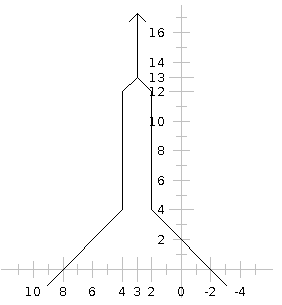
\includegraphics[scale=0.5]{../images/thermA.png}
\end{center}

In this case, $\ell(G) = 10 \leq 100$ and $\ell(\Gm{^{L_1}}) = \ell(\Gm{^{R_1}}) = 0 \leq 200$ and $\ell(\Gm{^{L_2}}) = \ell(\Gm{^{R_2}}) = 24 \leq 200$. The boiling point bound the theorem provided for $S$ is loose for \Gm{}. However, it is unclear if that is because the confusion intervals that define the class are also too lose or if the bound itself is large.

Let $S_*$, now, be the class given by $\{G : \ell(G)\leq10, \ell(G^L)\leq24, \ell(G^R)\leq24\}$. From the analysis of the previous paragraph, \Gm{\in S_*}. However, in this case, the confusion intervals of \Gm{} are tight in respect to the ones that define the class. From the theorem $\forall G \in S_*,\; BP(G) \leq 29$. The bound is tighter for \Gm{} but is still loose, which may lead to the belief that this bound is loose in general.

In order to verify whether the bound is in fact loose, it would bee needed to show the following, or something similar:
$$
\forall S,\;\exists x\in SN,\; x>0\;|\; \underset{G\in S}{max}BP(G) \leq BP(S) + x
$$

To dismiss the idea, however, it could be shown:
$$
\exists G \in S_*\;|\;\not\exists x>0,\; BP(G)\leq BP(S)+x
$$

Starting out with the previous example, take $\tilde{G} = \gam{\gam{28}{4}}{\gam{2}{-22}}$. The temperature is, of course, the same as before, 13. However, the Left and Right slant may be moved, since $\ell(\tilde{G}) = 2$. Take \Gm{_+=\gam{\gam{36}{12}}{\gam{2}{-22}}}, result of shifting the left slant to the left, while maintaining the left confusion interval.

\begin{center}
\begin{tabular}{cc}
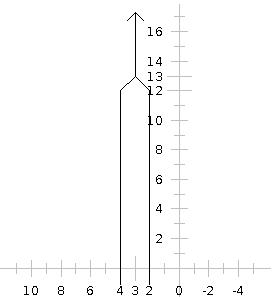
\includegraphics[scale=0.5]{../images/gtherm.png} & 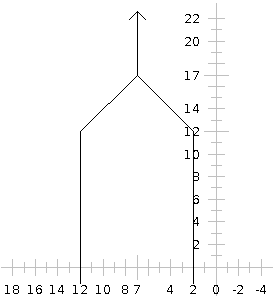
\includegraphics[scale=0.5]{../images/gplus.png} \\
$\tilde{G}$ & \Gm{_+} \\
\end{tabular}
\end{center}

The temperature 17 is higher than the initial one but is still far away from the desired 29. However, it is still possible to increase it more. The boiling point of left and right slants are 12, and, for this reason, the oblique line in the thermograph start at $t=12$. Making the left and right games hotter would increase the overall temperature, but increasing the confusion interval is not allowed as it is desired that the resulting game belongs to the class $S_*$.

Since the thermographs of \Gm{^{L/R}} are made of two oblique lines, making part of the lines straight would increase their temperature. One way of doing it is changing \Gm{^L} to \gam{\gam{60}{36}}{12}. The temperature of
\Gm{_-=\gam{\gam{\gam{60}{36}}{12}}{\gam{2}{\gam{-22}{-46}}}} is 23. To simplify further analysis, take \Gm{_1 = \gam{\gam{\gam{53}{29}}{5}}{\gam{{-}5}{\gam{-29}{-53}}}}, result of centering \Gm{_-} at 0. Notice that \Gm{_1 = \pm\gam{\gam{53}{29}}{5}}.

\begin{center}
	\begin{tabular}{cc}
		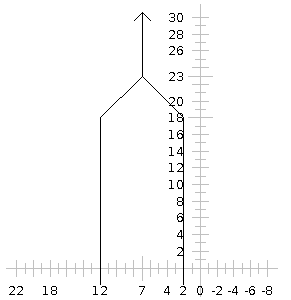
\includegraphics[scale=0.5]{../images/gminus.png} & 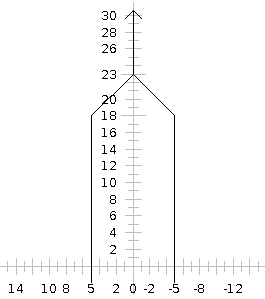
\includegraphics[scale=0.5]{../images/gone.png} \\
		\Gm{_-} & \Gm{_1} \\
	\end{tabular}
\end{center}

Following the idea of making one of the slants of \Gm{^{L/R}} straighter in order to increase their temperature, it is possible to keep increasing the temperature of \Gm{}. Consider the following sequence of games is $S_*$:

\begin{center}
	\begin{tabular}{c|c|c}
		i & \Gm{} & $t(G)$	\\
		\hline
		0 & $\pm$ \gam{29}{5} & 17 \\
		1 & $\pm$ \gam{\gam{53}{29}}{5} & 23 \\
		2 & $\pm$ \gam{\gam{\gam{77}{53}}{29}}{5} & 26 \\
		3 & $\pm$ \gam{\gam{\gam{\gam{101}{77}}{53}}{29}}{5} & 27.5 \\
	\end{tabular}\\
	\vspace{0.3cm}$\cdots$
\end{center}

The result that the temperature of games in this sequence increases and converges to 29 is desired, but it must be proved. The following proof is general for all sequence of games made in the likes of the sequence above.

\textit{Proof:} \todo{I made the proof -- revise}
\begin{list}{}{}
	\item[$\rightarrow$] Each term of the sequence increases the length of the straight segment of the left option of \Gm{^L} by $\frac{\ell(G^L)}{2^{i+1}}$.
	\item[ ] [Via Induction]
	\item[ ] Base case: $i=1$. Let $\Gm{=\gam{\gam{a + 2\ell(G^L)}{a+\ell(G^L)}}{a}}$. The right trajectory, $\rho$, of \gam{a + 2\ell(G^L)}{a+\ell(G^L)} is oblique until $t=\frac{\ell(G^L)}{2}$. Therefore the left trajectory, $\lambda$, of \Gm{} is straight until $\frac{\ell(G^L)}{2}$. At $t=\frac{\ell(G^L)}{2}$, the right trajectory is at the $a + \frac{\ell(G^L)}{2}$ x-coordinate. Since both trajectories are oblique above this temperature, they cross at the point $(a + \frac{3\ell(G^L)}{4},\; \frac{3\ell(G^L)}{4})$. Therefore, temperature was increased by $\frac{\ell(G^L)}{2}$.
	\item[ ] Induction Hypothesis: $i=k$. Let 
	$$
	\Gm{=\gam{
			\gam{
				\gam{
					\gam{\ldots
						\gam
							{a + (k+1)\ell(G^L)}
							{a + k\ell(G^L)}
						}
						{\ldots}
					}
					{a + 2\ell(G^L)}
				}
				{a+\ell(G^L)}
			}
			{a}
		}
	$$
	Let $b = a + \ell(G^L)$. It is possible to rewrite $G$ so that:
	$$
	\Gm{=\gam{
			\gam{
				\gam{
					\gam{\ldots
						\gam
						{b + k\ell(G^L)}
						{b + (k-1)\ell(G^L)}
					}
					{\ldots}
				}
				{b+\ell(G^L)}
			}
			{b}
		}
		{a}
	}
	$$
	Using the inductive hypothesis on:
	$$
	\Hm{=
			\gam{
				\gam{
					\gam{\ldots
						\gam
						{b + k\ell(G^L)}
						{b + (k-1)\ell(G^L)}
					}
					{\ldots}
				}
				{b + \ell(G^L)}
			}
			{b}
	}
	$$
	The left slant of $\Hm^L$ has a straight segment of size $\sum\limits_{i=1}^{k-1} \frac{\ell(G^L)}{2^{i+1}}$. Since the right option of $H^L$ is a number, $BP(H^L)= \sum\limits_{i=1}^{k-1} \frac{\ell(G^L)}{2^{i+1}} + \frac{\ell(G^L) - \sum\limits_{i=1}^{k-1} \frac{\ell(G^L)}{2^{i+1}}}{2}$. Therefore, $BP(H^L)= \frac{\ell(G^L) + \sum\limits_{i=1}^{k-1} \frac{\ell(G^L)}{2^{i+1}}}{2} = \sum\limits_{i=1}^{k} \frac{\ell(G^L)}{2^{i+1}}$. Since the right slant of $H^L$ is oblique with size equals to the given temperature, then the left slant of $H$ is straight with the same size. Since $H = G^L$, then the inductive step is indeed correct.
	\item[$\rightarrow$] Each term of the sequence increases the length of the straight segment of the right option of \Gm{^R} by $\frac{\ell(G^R)}{2^{i+1}}$.
	\item[ ] The proof is analogous.
	\item[$\rightarrow$] If both the left option of \Gm{^L} and the right option of \Gm{^R} have their straight length increased by $l$, then so does \Gm{}.
	\item[ ] As seen before, $t(G) = T^L_V + T^L_O$. Since $\forall i,\; G_i = \tilde{G_i}$ and that increasing both trajectories straight segments does not affect the size of the oblique segments, it is possible to conclude that the temperature of the whole game will increase exactly $l$. Since, again, the size of the oblique segment does not change than the size of the straight segment increased by $l$.
	\item[$\rightarrow$] The temperature of the games in this sequence converges to the proposed boiling point, while always being elements of the initial class $S$.
	\item[ ] Notice that $RS(G^L)$ and $LS(G^R)$ remain the same across all iterations, and that $RS(G^L) - LS(G^R) = \ell(G)$, it is clear that $\forall i, \ell(G_i) = \ell(G)$.
	\item[ ] Notice that the observation above is valid for \Gm{^L} and \Gm{^R}.
	\item[ ] The previous two observations show that every game in the sequence belongs to $S$.
	\item[ ] The initial height is $\frac{\ell(G)}{2} + \frac{\ell(G^L)}{2}$. From the first three points of the proof, at each iteration $i$ the straight segments of $\lambda(G)$ and $\rho(G)$ increase by $\frac{\ell(G^L)}{2^{i+1}}$, $\ell(G^L) = \ell(G^R)$. Since increasing the straight segments of $\lambda(G)$ and $\rho(G)$ does not affect the size of the oblique segments, then $t(G)$ increases by that amount at each iteration.
	\item[] \hspace{-1cm} $t(G_k) = \frac{\ell(G)}{2} + \frac{\ell(G^L)}{2} + \sum\limits_{i=1}^{k} \frac{\ell(G^L)}{2^{i+1}} = \frac{\ell(G)}{2} + \sum\limits_{i=1}^{k} \frac{\ell(G^L)}{2^{i}} = \frac{\ell(G)}{2} + \ell(G^L) - \frac{\ell(G^L)}{2^k} \leq \frac{\ell(G)}{2} + \ell(G^L)$.
\end{list}

The sequence of games, then, shows that the given bound is not loose. In fact, it shows that the bound is optimal for some cases. It is worth mentioning that, although this section follows the aforementioned paper, the proof above is original. The paper does convey the strategy and the regard about the optimality of the bound but the proof of convergence is skipped. Although long and with many symbols, the proof is quite simple and might be considered trivial.

An interesting way to complete and put to practice the analysis of the theorem is to show it can be used to characterize a pattern of domineering boards. To use the bound all games following the pattern must belong to a class, based on the confusion interval restrictions, like before.

When bounding `$2\times n$ snakes' boards, the thesis and the featured papers diverge. Probably in the year between the publish of the thesis and the paper the technique was refined, resulting in the thesis bringing a bound of $5$ to the temperature and the paper reducing it to $3$. The proof brought to this text will show the point of divergence. Before showing the proof, another necessary definition and lemma are provided.

A `snake' board, same adjective used in ``Kim's snakes" from the previous chapter, is a board without any $2\times 2$ subgrid. A `$2\times n$' snake is a snake that fits in a $2\times n$ board. It is possible to use the term `snake fitting in a $2\times n$ board', and this means that the board is a snake that can be folded such that it becomes a `$2\times n$' snake with the same value.

The lemma is: Let $\epsilon$ be any infinitesimal and \Gm{} be a hot game. If for all left options \Gm{^L}, $n$ is a number such that $G^L - G - n +\epsilon \leq 0$, then $\ell(G) \leq n$. The proof is simple, again.
\begin{align*}
	\ell(G) =& LS(G) - RS(G) \\
	=& RS(G^L) + LS(-G) \\
	\leq& LS(G^L - G) \\
	\leq& n
\end{align*}

It is clear that $LS(G) = RS(G^L),\; RS(G) = - LS(-G)$, but the second equation is there to help visualize the first inequation. The last inequation is true because $G^L - G + \epsilon \leq n \longrightarrow LS(G^L-G)\leq n$, explained amid the discussion in the beginning of this section. The first inequation is true because $G^L - G = \gam{G^{LL}-G^L}{G^{LR}-G^R}$, meaning that $LS(G^L-G)$ derives from a game $\Hm = \Gm{^L_+} - \Gm{_-}$. In particular, it is possible to take \Gm{^L_+} to be a game that defines the right stop for \Gm{^L} and $-\Gm{_-}$ the game that defines the left stop for $-G$, and, therefore, the inequality is true.

The meaning of this lemma is that if it is possible to bound the value of the game to the left, or to positive side, then it is possible to bound the confusion interval. This is a weaker result compared to the previous but it is one that connects the stops with the confusion interval so it is extremely useful.

Now it is possible to characterize some domineering boards. \textit{The temperature of snakes fitting a $2\times n$ board is at most $3$.} The proof consists of showing that $\ell(G), \ell(G^L), \ell(G^R) \leq 2$, by the means of showing that for $\Hm = G \lor G^L \lor G^R \rightarrow H^L -H -2 \leq 0$ and using the lemma above.

Considering the case $H = G^R$, \Hm is a two component board, so it is possible to separate them in distinct games. Let $-H = -G^R = -G_1 - G_2$. $H^L$ on the other hand is \Gm{^R} with the addition of a left move. The only cases a left move does not exist in \Gm{^R} is if \Gm{} is one of the following:

\begin{figure} [!ht]
\begin{center}
\begin{tikzpicture}
\draw[] (0,0) rectangle ++(0.3,0.3);
\draw[] (0,0.3) rectangle ++(0.3,0.3);
\end{tikzpicture}
\hspace{1cm}
\begin{tikzpicture}
	\draw[] (0,0) rectangle ++(0.3,0.3);
	\draw[] (-0.3,0) rectangle ++(0.3,0.3);
	\draw[] (0,0.3) rectangle ++(0.3,0.3);
\end{tikzpicture}
\hspace{1cm}
\begin{tikzpicture}
	\draw[] (0,0) rectangle ++(0.3,0.3);
	\draw[] (-0.3,0) rectangle ++(0.3,0.3);
	\draw[] (0,0.3) rectangle ++(0.3,0.3);
	\draw[] (0.3,0.3) rectangle ++(0.3,0.3);
\end{tikzpicture}
\end{center}
\end{figure}

In all the cases above, the temperature is below 3, so it is not a problem. Without losing generality, let \Gm{_1} be a component where there is a right move, and let the initial left move be any such move in \Gm{_1}, therefore, $H^L = G_1^L + G_2$. Now it is clear that this case can be reduced to the case $H = G_*$, with \Gm{_*} a smaller board than \Gm{}:

$$
H^L - H = G_1^L + G_2 - G_1 - G_2 = G_1^L - G_1
$$

Repeating the process with $H = G^L$, $-H = -G^L = -G_1 - G_2$ and $H^L = G_1^L + G_2$. The only cases \Gm{_1^L} does not exist is if
\Gm{=\begin{tikzpicture}
		\draw[] (0,0) rectangle ++(0.3,0.3);
		\draw[] (0.3,0) rectangle ++(0.3,0.3);
	\end{tikzpicture} \text{ or } \begin{tikzpicture}
	\draw[] (0,0) rectangle ++(0.3,0.3);
	\draw[] (0.3,0) rectangle ++(0.3,0.3);
	\draw[] (0.3,0.3) rectangle ++(0.3,0.3);
\end{tikzpicture}} and both of them have temperature lesser than 3. Again it is clear that this case can also be reduced to the case $H = G_*$:

$$
H^L - H = G_1^L + G_2 - G_1 - G_2 = G_1^L - G_1
$$

Therefore, if $\ell(G) \leq 3$ then the confusion interval of both option are also smaller than 3. To prove that $G^L - G - 2 \leq 0$ it is shown a winning strategy for right in $G^L - G - 2$, which shows that the position is negative. First notice that $-G$ is \Gm{} flipped so that it fits in a $n\times 2$ board, but a useful way, that is used in this proof, to consider $-G$ is Left playing on the horizontal and Right playing on the vertical.

To help visualize the strategy for this case, let the `shadow' of a move be the same cells that the move occupied, but in the opposing board. Also the board resultant from play in $G^L$ is called the original board and the board resultant from play in $-G$ is called the opposing board. For instance:

\begin{figure}[h]
	\centering
	\begin{subfigure}{0.17\linewidth} \centering
		\begin{tikzpicture}
			\node (title) at (0.45,1) {\Gm{^{L/R}}};
			\draw[] (0,0) rectangle ++(0.3,0.3);
			\draw[fill=gray] (0.3,0.3) rectangle ++(0.3,0.3);
			\draw[] (0.6,0.3) rectangle ++(0.3,0.3);
			\draw[fill=gray] (0.3,0) rectangle ++(0.3,0.3);
			\node[] at (1.3,0.3){$\cdots$};
			\node[] at (-0.4,0.3){$\cdots$};
		\end{tikzpicture}
		\caption*{\hspace{0.1cm}Orginal move\newline Original board}
	\end{subfigure}
	\hspace{1cm}
	\begin{subfigure}{0.17\linewidth} \centering
		\begin{tikzpicture}
			\node (title) at (0.45,1) {-$G$};
			\draw[] (0,0) rectangle ++(0.3,0.3);
			\draw[pattern=north west lines,pattern color=gray] (0.3,0.3) rectangle ++(0.3,0.3);
			\draw[] (0.6,0.3) rectangle ++(0.3,0.3);
			\draw[pattern=north west lines,pattern color=gray] (0.3,0) rectangle ++(0.3,0.3);
			\node[] at (1.3,0.3){$\cdots$};
			\node[] at (-0.4,0.3){$\cdots$};
		\end{tikzpicture}
		\caption*{\hspace{0.15cm}Shadow move\newline Opposing board}
	\end{subfigure}
\end{figure}

In the game $G^L -G -2$, if Right plays first, he/she simply has to mimic each and every move Left made by playing the shadow move, maintaining $-2$ intact, starting with the move already played in \Gm{^L}. If, instead Left goes first, he/she can play one of two options. The first is to play a move that does not intersect the shadow of the previous move. In this case, right must play the shadow of either the first or the second move.

Essentially, this first case maintains the original conditions while reducing the board size. This case leads $G^{L_*} -G -2$ to $G^{L_*L} -G^{L_*} -2$, which, by taking $H = G^{L_*}$, is $H^{L} -H -2$. Therefore the only worrisome Left move is one that intersects the shadow of the initial move. This move is not exactly the shadow move because in the opposing board Left moves in another orientation. After Left's move, Right must move on the $-2$ component, taking it to $-1$.

Now, Left can, again, play a move that does not intersect any of the shadows, but this would be met by the same strategy as before, so Left must play a move that intersects a shadow. However, Left cannot move intersecting the shadow of the previous move, because the initial move would be adjacent to this third move and since the mover are both vertical, a $2\times 2$ subgrid would have to exist. The only shadow Left can intersect is that of the first move, playing on the opposing component again. After Left's third move, right plays on the $-1$ component.

At this time, Left can no longer play on any shadows, so he/she cannot avoid Right's strategy and will eventually lose. Therefore, if \Gm{} is a snake fitting in a $2\times n$ grid, then $G^L - G -2 < 0$. This means that $\ell(G),\ell(G^L),\ell(G^R) \leq 2$. By using the bound result, in turn, it means that $t(G) \leq 3$. 

This result from the 2019 paper is different, as stated before, from the 2018 thesis because the first part of the proof, that shows the cases $H=G^L,G^R$ can be reduced to the case $H=G$, was missing. Instead the original text only showed that the confusion intervals of $G^L,G^R$ were smaller than 4. This second result is clear because both $G^L$ and $G^R$ are made of two components that are snakes fitting in $2\times n$ grids. As the text shows that such a snake has the confusion interval smaller or equal to 2, then two snakes have that interval smaller or equal to 4.















    
% Conclusion
    \chapter{Unexplored games and final remarks}
    Combinatorial game theory is a new field in mathematics that was initially found in the blend of recreational mathematics, combinatorics and number theory. While the initial focus is finding strategies to play better and win games, the developments it prompted in other areas of mathematics have their own place, independent of the initial purpose. The Surreal Numbers form a class with many interesting properties and found much enthusiasm for that reason, not because it was necessary to analyze games.

However, the surreal numbers inevitably carry the simplicity inherited from the mathematical plays it was created/discovered for. It is commonplace to learn how to breach the gap between rational and real numbers only in superior education, partially because any of the common constructions involves operations and procedures not used in school. Surreal Numbers give for free the construction of real numbers from its few and simple rules. Not only the reals, but a definition of positivity and negativity that dismisses comparison, a common method for the creation of all the numbers, new numbers and, at last, a direct way of visualizing each number with RB-Hackenbush games. Numbers are the main building block the text used to analyze games.

The non-numbers, a name used in this text for games with temperatures, are the remaining games and required more elements and concepts to be understood. The thermograph, or the form commonly used to visualize temperature, options, stops and boiling points, is extensively analyzed and the text presents one of the most recent related results.

The reader that understands all the featured topics and is able to replicate calculations and results to games other than the mentioned might carry the false belief that understands all of combinatorial game theory. This text, however, only describes the class of partisan games leaving many variations even unmentioned. Not only the focus is specific, but also not all perspectives necessary to tackle the problem of finding the best move are visited.

These information serves to show that there is much more to the field, not that little progress understanding it was made. In fact, it is fair to state that the classes of games discussed in the text are the more complicated ones and many of the definitions apply to other classes.

Both in the results discussed and the ones omitted there is a common trend in this field. The definitions are always simple, but powerful enough to allow many questions, and, although there are many open questions, the proofs are and solutions are simple as well. The procedure to build all dyadic rationals in domineering boards, for example, is based on a theorem provable in two lines of text and applying it is the simplest of ways. Although its explanation is simple, it remained open for years and the resulting pattern is not something that would be found before the proof.

Finding the upper bound to temperature is another case where the question remained open for long, but the strategy used to answer is simplicity: it consists only of listing and manipulating properties of the thermographs.That is not to say that the bounding of temperature is completely solved but the progress made used simple steps.

From this perspective combinatorial game theory is a beautiful field in mathematics. The definitions it is based upon are extremely few in number and very simple in form, but they allow proving more complex problems in a uncomplicated manner. However, in this text, one of the unvisited places in the field is computational complexity. In practice, calculating values is not an easy problem.

The other featured aspect skipped is the variety of forms combinatorial games might take, because the text only deals with partisan games played on normal conditions. The remaining contains a brief description of these two skipped problems and points toward texts on th respective subjects. This chapter, that finalizes the text, also addresses a few of the next steps studying or researching the field and ends with a personal reflection on the learning, implementing and writing experiences involved in this work.


\subsection*{Undeveloped Pieces}

\subsubsection*{Complexity}

The text repeatedly made the case that most concepts are simple in Combinatorial Game Theory. It said, for example, that the method used to find the number a game is equal to is straight-forward. However this hides an important factor.

Either calculating the number or building a thermograph requires, first, traversing the game tree. Traversing this tree and calculating the values is simple enough, but it is slow. And it is slow because this tree quickly becomes large. For example, consider the following game of Domineering.

\begin{center}
\begin{tikzpicture}
\draw[step=0.5cm,color=gray] (-1,-1) grid (1,1);
\newcounter{mycount}
\setcounter{mycount}{`A}
\foreach \y in {+0.75,+0.25,-0.25,-0.75}
\foreach \x in {-0.75,-0.25,0.25,0.75}
\node at (\x,\y) {\addtocounter{mycount}{1}};
\end{tikzpicture}
\end{center}

There are, of course, 25 squares, which means that at most 12 moves might be made and in addition, some of these moves might be equivalent, so they do not have to be computed multiple times. It happens that only 604 nodes, or different position, may be reached\cite{1}. In a $6\times 6$ board it jumps to $17,232$ and in $7\times 7$ and $8\times 8$ board it goes to $408,260$ and $441,990,070$ nodes. Although these results are from 1998, results on larger boards took many years and only in 2016 a result for $11 \times 11$\cite{2} board was found, but abandoning a naive building of a game tree. The game tree of a $9\times 9$ board has around 25 trillion nodes.

If not clear at first it should be now that there is no known form of calculating values for games in polynomial time is respect to their sizes. The question, then, is in what class of problems it fits. It happens that many of the games are known to be PSPACE-complete and some are known to be EXPTIME.

There is of course much more to be said an it is another very interesting topic. A good starting point is \textit{Playing Games with Algorithms: Algorithmic Combinatorial Game Theory}\cite{3}. The thesis \textit{Games, Puzzles, and Computation} is more extensive, covering different classes of games, but may be more complex. Regardless of the suggested texts, there is a large amount of great books on complexity theory.

\subsubsection*{Other games}

By looking at the definition of combinatorial games given in the beginning of section 2, it is easy to come up with games that do not fit well the class of games studied, the short games. One clear example is the game of chess, because there are ties and there are drawn positions.

However, games like chess are not the only class of games that behave differently. Consider G-Hackenbush, a variation of RB-Hackenbush, in which both blue and red edges are replaced by green ones. Green edges may be removed by either player, meaning that both players have the same available moves regardless of the position. The class of games that follow this property is called Impartial Games.

Impartial games were the first games studied, previously to the consolidation of the modern form of the field. They have an interesting property of being reducible to an instance of a game of Nim. 

Games like chess, on the other hand, are not so simple. there are more classes of results than short games, which allows games to become more complex. Such games benefit from knowing short game's theory but do require further concepts. A good place to start is the corresponding chapter in the book \textit{Combinatorial Game Theory}.


\subsection*{Post-Match}

The choice of Combinatorial Game Theory as subject was an extremely fortunate decision. This field triggered the feeling of uncovering something beautiful hidden in plain sight. I believe the book \textit{Winning Ways} played a role in that due to the presentation I became found of, but I do considered there is inherent beauty in the field.

I believe the simplicity of everything about it is something to awe. This is the most important reason why this thesis ended up being about it and not some other subject. The first step in this directions was a great interest in the games of Chess, Shogi and Go. The first idea I had was to develop heuristics to find shortest paths in the game of chess, and possibly extend that to other games using more general graph theory.

During this period I started reading articles and scrolling through books and that quick led me into the field of Combinatorial Game Theory. The book \textit{Winning Ways} is one of the canonical references and I luckily started with that. This choice led me to a year of great learning experiences, in many areas, and personal maturing.

Learning and writing about the topics of this text was the most important activity to conclude my Bachelor's Thesis, but there are other subjects I studied in the process that went unmentioned in the text. I am grateful for those too, as I got to develop my understanding of real analysis and complexity theory further than I would normally, for example. This year was also the one of we had the corona virus widespread and, hopefully, the last year we have to partake isolation and health/economic insecurity.

I had only handful of on-campus classes and that required me, and most of the world, to adapt to new circumstances. While it did not effect the content of this text directly, it greatly impacted the world we live in. Frequently during the year I found myself struggling to concentrate and in a general bad mental state. The consistent work it took really helped keeping me on track. Another factor that can not go unmentioned is the help of my advisor.

José Coelho kept regularly meeting me almost every week during this year. That helped a lot keeping me in check and I am extremely thankful of the dozens of hours we spent talking and discussing the most varied subjects. In the times I did not have work to show he was understanding and his willingness to help pushed me further and further.












    
    
% Bibliography
    \phantomsection
    \nocite{*}
    \addcontentsline{toc}{chapter}{References}%
    \bibliography{bibliography}
    
    \appendix
    \chapter{CGSuite}
    \textcolor{red}{The final sections of your thesis are the appendices. Each appendix should be lettered (A, B, etc.,) and should consist of detailed information that is interesting but not essential to the main thrust of your findings section.\\
The appendices should be in the order that they are referred to in the main text. For instance, if Appendix A refers to something on page 25 and Appendix B refers to something on page 15, the appendices need to be re-lettered. This inconsistency occurs when text is moved around or inserted.)}

    

\end{document}
%----------------------------------------------------------------------------------------------------%
